% Options for packages loaded elsewhere
\PassOptionsToPackage{unicode}{hyperref}
\PassOptionsToPackage{hyphens}{url}
\documentclass[
  10pt,
]{article}
\usepackage{xcolor}
\usepackage[margin=1in]{geometry}
\usepackage{amsmath,amssymb}
\setcounter{secnumdepth}{-\maxdimen} % remove section numbering
\usepackage{iftex}
\ifPDFTeX
  \usepackage[T1]{fontenc}
  \usepackage[utf8]{inputenc}
  \usepackage{textcomp} % provide euro and other symbols
\else % if luatex or xetex
  \usepackage{unicode-math} % this also loads fontspec
  \defaultfontfeatures{Scale=MatchLowercase}
  \defaultfontfeatures[\rmfamily]{Ligatures=TeX,Scale=1}
\fi
\usepackage{lmodern}
\ifPDFTeX\else
  % xetex/luatex font selection
\fi
% Use upquote if available, for straight quotes in verbatim environments
\IfFileExists{upquote.sty}{\usepackage{upquote}}{}
\IfFileExists{microtype.sty}{% use microtype if available
  \usepackage[]{microtype}
  \UseMicrotypeSet[protrusion]{basicmath} % disable protrusion for tt fonts
}{}
\makeatletter
\@ifundefined{KOMAClassName}{% if non-KOMA class
  \IfFileExists{parskip.sty}{%
    \usepackage{parskip}
  }{% else
    \setlength{\parindent}{0pt}
    \setlength{\parskip}{6pt plus 2pt minus 1pt}}
}{% if KOMA class
  \KOMAoptions{parskip=half}}
\makeatother
\usepackage{longtable,booktabs,array}
\usepackage{caption}
\captionsetup[table]{skip=6pt}
\newcounter{none} % for unnumbered tables
\usepackage{calc} % for calculating minipage widths
% Correct order of tables after \paragraph or \subparagraph
\usepackage{etoolbox}
\makeatletter
\patchcmd\longtable{\par}{\if@noskipsec\mbox{}\fi\par}{}{}
\makeatother
\usepackage{graphicx}
\makeatletter
\newsavebox\pandoc@box
\newcommand*\pandocbounded[1]{% scales image to fit in text height/width
  \sbox\pandoc@box{#1}%
  \Gscale@div\@tempa{\textheight}{\dimexpr\ht\pandoc@box+\dp\pandoc@box\relax}%
  \Gscale@div\@tempb{\linewidth}{\wd\pandoc@box}%
  \ifdim\@tempb\p@<\@tempa\p@\let\@tempa\@tempb\fi% select the smaller of both
  \ifdim\@tempa\p@<\p@\scalebox{\@tempa}{\usebox\pandoc@box}%
  \else\usebox{\pandoc@box}%
  \fi%
}
% Set default figure placement to htbp
\def\fps@figure{htbp}
\makeatother
\setlength{\emergencystretch}{3em} % prevent overfull lines
\providecommand{\tightlist}{%
  \setlength{\itemsep}{0pt}\setlength{\parskip}{0pt}}
% Generated by scripts/paper_to_latex.py; submitted with the bundle.
% Software Heritage identifiers are 50 unbroken hexadecimal characters and
% appear both inline and in a verbatim block. Without these the inline one runs
% 123pt past the right margin and the block 66pt.
\usepackage{fvextra}
\DefineVerbatimEnvironment{verbatim}{Verbatim}{breaklines=true,breakanywhere=true}
\usepackage{seqsplit}
\setlength{\emergencystretch}{4em}
\usepackage{bookmark}
\IfFileExists{xurl.sty}{\usepackage{xurl}}{} % add URL line breaks if available
\urlstyle{same}
% fallback for those not using the hyperref driver hyperxmp:
\makeatletter
\@ifundefined{xmpquote}{\newcommand{\xmpquote}[1]{#1}}{}
\makeatother
\hypersetup{
  hidelinks,
  pdfcreator={LaTeX via pandoc}}

\author{}
\date{}

\begin{document}

{
\setcounter{tocdepth}{3}
\tableofcontents
}
\section{Auditing a quantum-classical kernel comparison: a
pre-registered null and what its own artefact will
support}\label{auditing-a-quantum-classical-kernel-comparison-a-pre-registered-null-and-what-its-own-artefact-will-support}

\textbf{GENERATED FILE. Do not edit.} Assembled by
\texttt{scripts/assemble\_paper.py} from the section files listed below.
Edit a section and re-run; \texttt{-\/-check} fails if this file has
drifted from its sources.

Assembled 2026-10-21T00:15:46+00:00 at commit \texttt{c7d5dc6}.

{\def\LTcaptype{none} % do not increment counter
\begin{longtable}[]{@{}lll@{}}
\toprule\noalign{}
section & source & sha256 \\
\midrule\noalign{}
\endhead
\bottomrule\noalign{}
\endlastfoot
Abstract & \texttt{docs/paper-abstract.md} &
\texttt{e8de5d9407875e8c} \\
1 & \texttt{docs/paper-introduction.md} & \texttt{7e7279f51ce61f94} \\
2 & \texttt{docs/paper-background.md} & \texttt{b77857d2ab111f69} \\
3 & \texttt{docs/paper-design.md} & \texttt{248f7f0f316ea1cf} \\
4 & \texttt{docs/paper-results.md} & \texttt{b32aecd493a5dce3} \\
5 & \texttt{docs/paper-protocol.md} & \texttt{fde9712da551c93d} \\
6 & \texttt{docs/paper-discussion.md} & \texttt{18453af3c95068b7} \\
7 & \texttt{docs/paper-deviations-pointer.md} &
\texttt{1bfa12527bc78e11} \\
References & \texttt{docs/paper-references.md} &
\texttt{958b0237e15ec45f} \\
\end{longtable}
}

\begin{center}\rule{0.5\linewidth}{0.5pt}\end{center}

\section{Abstract}\label{abstract}

Can a cheap pre-training quantity tell a practitioner not to bother with
a quantum kernel? We pre-registered that question on imbalanced business
tabular data, customer churn and credit-card fraud, across 360 units:
three mappings, five qubit counts, three training sizes, four quantum
settings, twenty seeds, statevector simulation only.

Neither primary cell shows a quantum advantage. On churn both endpoints
reject \emph{against} the quantum kernel, a median deficit of 0.0659
normAP, clearing its true minimum detectable effect by 1.31x. On fraud
the test does not reject and is reported as a bound: an advantage above
0.0063 normAP is excluded at 80\% power.

For the geometric difference the registered rule returned \textbf{no
verdict}, because no regularisation column is free of ceiling breaches.
That is the rule declining to speak, not a finding that no relationship
exists: at the largest regularisation the null \emph{is} rejected in the
predicted direction, yet accounts for 2.9\% of rank variance and
reverses sign across the sweep, so the quantity is not usable as the
screen it is offered as. A third rule, the source's own and one no one
had run, selects no parameter at all on 76.5\% of units, returning
nothing to test.

Seventeen deviation records govern; the recovered pre-rewrite history is
now published, so every stored commit identifier resolves.

\begin{center}\rule{0.5\linewidth}{0.5pt}\end{center}

\section{Section 1 --- Introduction}\label{section-1-introduction}

A quantum-classical kernel comparison can be run carefully, pass every
test its authors wrote, and still not support the claim made from it.
The ways such a comparison fails are mostly not visible in its results:
a metric compared across two different nulls, a difference below the
arithmetic resolution of the pipeline, power measured on the wrong
pairs, an asymmetric quantity carried into code with its arguments the
wrong way round. None of these shows up as an error. Each shows up as a
number.

This paper is about what a published artefact lets a reader establish,
worked through a pre-registered comparison that was built to answer a
different question and, in answering it, kept finding that the question
behind it was whether anyone could check.

\begin{center}\rule{0.5\linewidth}{0.5pt}\end{center}

\subsection{1.1 The registered question}\label{the-registered-question}

Huang et al.'s geometric difference is used as a screen: compute a cheap
quantity from two kernel matrices before training, and learn whether a
quantum kernel could outperform a classical one on this data. The
practitioner's version is narrower and more useful --- can a cheap
number tell me \textbf{not to bother}?

This study registered that question on imbalanced business tabular data,
where the claim matters commercially and where the literature's
benchmarks mostly are not: Telco customer churn and credit-card fraud,
360 pre-registered units across three feature mappings, five qubit
counts, three training sizes and four quantum settings, twenty seeds
each.

\begin{center}\rule{0.5\linewidth}{0.5pt}\end{center}

\subsection{1.2 What this paper reports}\label{what-this-paper-reports}

\textbf{A screen that is not usable, within its tested scope.} On those
360 units the registered decision rule returns no verdict, because no
regularisation column is free of ceiling breaches under any of three
\(\lambda\) rules evaluated --- a rule declining to speak, not a finding
that no relationship exists. The third of those rules is the one Huang's
own source prints, and it turned out not to select a \(\lambda\) at all
on \textbf{76.5\%} of the units: on 81.3\% of them his \(\lambda\) rule
and his \(\sqrt{N}\) ceiling cannot both be satisfied. Neither this
study nor the peer-reviewed paper that inherited the quantity had ever
run it. At \(\lambda\) = 0.1, the only column where all 360 units
survive, the null \emph{is} rejected and in the predicted direction: rho
= +0.17, p = 1.1e-03. That relationship accounts for \textbf{under three
percent of the rank variance} and \textbf{reverses sign} across the
regularisation sweep --- to -0.38 at \(\lambda\) = 1e-3 --- so what it
appears to say depends on a parameter the practitioner chooses. A
quantity explaining three percent of rank variance, whose sign moves
with a free parameter, cannot tell a practitioner not to bother.
Alongside it, no quantum advantage at either primary cell: on churn a
measured classical advantage, on fraud an exclusion bound.

\textbf{An audit procedure that separates three things published work
routinely merges}: a measurement, a refusal, and an unsupported claim. A
measurement says what a quantity is. A refusal says the file cannot
answer a question and names which. An unsupported claim is an assertion
its own artefact does not license. The procedure's output is mostly
refusals, and the paper is explicit that a refusal is not a finding
about the audited work.

\textbf{A record format whose value is a property of the format.} A
results file carrying the fields in \S{}5.2 can be audited by a stranger
in seconds, without the pipeline that produced it, and the audit states
which questions that file cannot answer. This is the one claim here made
without qualification.

\textbf{Source-to-implementation checking, with results.} Reading two
papers at source rather than in rendering, and comparing against their
released code, established that an asymmetric quantity is introduced in
an appendix with its arguments reversed relative to the main text and
without relabelling, and that the reversal propagates into a
peer-reviewed paper whose equation, code and stated interpretation all
agree with one another. Applied to this project itself, the same
procedure established that \textbf{every one of its 15,120 result
records stores a code identifier no reader can resolve}.

\begin{center}\rule{0.5\linewidth}{0.5pt}\end{center}

\subsection{1.3 What this paper does not
claim}\label{what-this-paper-does-not-claim}

Stated here rather than left to the discussion, because each is a claim
a reader might reasonably expect and none is supported.

\textbf{Not that the geometric difference is invalid in general.} It was
measured on one grid, with one treatment of its regularisation
parameter, on two datasets, one of which is saturated at every training
size tested. A quantity can be uninformative where it was measured and
informative elsewhere, and nothing here separates those cases.

\textbf{Not that it carries no signal.} At the one breach-free
regularisation column the relationship is statistically detectable and
runs in the predicted direction. The claim above is about usability ---
an effect of that size, with that sign instability, cannot support a
go/no-go decision --- and not about absence.

\textbf{Not that the audit detects defects in other people's pipelines.}
On the one occasion these checks met records they were not designed
around, they produced one measurement and eight refusals and
\textbf{found no defect, nor were they looking for one}. Whether they
would detect an error in unfamiliar work is, on one case, unevidenced
either way.

\textbf{Not that the protocol is validated.} Every records-level and
kernel-level check was written after the defect it catches. The
instrument has needed repair seven times in public, three times because
the tool was wrong and four times because its authors stated something
their own data does not support. Two of the seven are the same lesson
twice: a superseded exclusion bound that the confirmatory script printed
for eleven days after the correction was written, pinned in place by a
regression test, and the registered adjudicator of grid adequacy, which
printed a verdict its own record had withdrawn for three weeks. Nothing
in the protocol caught either, because nothing in the protocol reads
this project's own analysis and reporting code.

\textbf{Not that the findings about published work are errors in their
conclusions.} They are statements that a claim cannot be checked from
the published artefact without going to source. In the orientation case
the ambiguity originates upstream of the authors who inherited it.

\begin{center}\rule{0.5\linewidth}{0.5pt}\end{center}

\subsection{1.4 How to read this}\label{how-to-read-this}

Section 2 establishes what the geometric difference is, what its bound
does and does not assert, and how its arguments compose --- the
derivation the rest depends on. Section 3 traces the registered design
and marks every subsequent amendment. Section 4 reports the results,
with its limitations in \S{}4.7. Section 5 is the protocol: what is
tooling, what is a reading procedure, what each costs, and \S{}5.6,
which argues against the contribution. Section 6 bounds what all of it
supports. Section 7 points at the deviation records, which govern
wherever they and the pre-registration disagree.

A reader with limited time and a sceptical disposition should read
\S{}5.6 and \S{}6.3 first. They are where this paper says what its
evidence will not carry.

\begin{center}\rule{0.5\linewidth}{0.5pt}\end{center}

\section{Section 2 --- Background: the geometric difference and its
ordered
arguments}\label{section-2-background-the-geometric-difference-and-its-ordered-arguments}

\textbf{Draft, 3 October 2026.} Written under the framing recorded in
D15.

This section states what the geometric difference is, what Huang's bound
does and does not claim, and what happens to both when an asymmetric
quantity is carried from a paper into code. Throughout, three things are
kept apart and labelled: \textbf{what a source states}, \textbf{what an
implementation does}, and \textbf{what this project verified by
comparing them}. That separation is not stylistic. The errors this
section documents live exactly in the gap between the three.

\begin{center}\rule{0.5\linewidth}{0.5pt}\end{center}

\subsection{2.1 The quantity}\label{the-quantity}

Huang et al.~introduce the geometric difference to answer a question
about \emph{model complexity} rather than about accuracy: given a
function a model with kernel K\(^{1}\) can represent, how much
complexity does a model with kernel K\(^{2}\) need to reproduce it?

\textbf{Source states} (arXiv:2011.01938, read from the e-print LaTeX;
see 2.6 for provenance). Equation (5):

\begin{quote}
g(K\(^{1}\) \(\|\) K\(^{2}\)) = sqrt( \(\|\) sqrt(K\(^{2}\))
(K\(^{1}\))\(^{-1}\) sqrt(K\(^{2}\)) \(\|\)\_\(\infty\) )
\end{quote}

with \(\|\)\(\cdot\)\(\|\)\_\(\infty\) the spectral norm and the
normalisation tr(K\(^{1}\)) = tr(K\(^{2}\)) = N, N the number of
training samples. The accompanying bound is

\begin{quote}
s\_\{K\(^{1}\)\} \(\le\) g(K\(^{1}\) \(\|\) K\(^{2}\))\(^{2}\) \(\cdot\)
s\_\{K\(^{2}\)\}
\end{quote}

where s\_K is the model complexity under kernel K.

Three properties follow from the printed definition and matter for
everything after.

\textbf{It is asymmetric.} The inverse falls on the first argument and
the outer square roots on the second. g(K\(^{1}\)\(\|\)K\(^{2}\)) and
g(K\(^{2}\)\(\|\)K\(^{1}\)) are different numbers, and nothing in the
notation prevents one being used where the other is meant.

\textbf{It is a necessary condition, not a sufficient one.} Source
states: \emph{``if the geometric difference is small, then a classical
ML method is guaranteed to provide similar or better performance''}, and
*``if g\_CQ is large we show that there exists a data set with s\_C =
g\(^{2}\)\_CQ s\_Q''* with the quantum model performing better. A large
g establishes that \textbf{some} dataset exists on which the quantum
model wins. It does not establish that any particular dataset is such a
dataset.

\textbf{It is bounded.} With the trace normalisation above, g cannot
exceed \(\sqrt{N}\). A value above that ceiling reports that the inverse
is under-regularised, not that the kernels are far apart.

The screening quantity is therefore \textbf{g(K\_C \(\|\) K\_Q)} ---
classical first, so the classical kernel is the one inverted --- and it
must be large for a quantum advantage to be possible at all.

\begin{center}\rule{0.5\linewidth}{0.5pt}\end{center}

\subsection{2.2 The regularised form, and a reversal inside the
source}\label{the-regularised-form-and-a-reversal-inside-the-source}

An exact inverse is unusable on an ill-conditioned Gram matrix, so the
regularised form is what anyone computes.

\textbf{Source states.} Appendix F, Equation (F19):

\begin{quote}
g\_gen = sqrt( \(\|\) sqrt(K\(^{1}\)) sqrt(K\(^{2}\)) (K\(^{2}\) +
\(\lambda\)I)\(^{-2}\) sqrt(K\(^{2}\)) sqrt(K\(^{1}\))
\(\|\)\_\(\infty\) )
\end{quote}

and (F20):

\begin{quote}
g\_tra = \(\lambda\) \(\cdot\) sqrt( \(\|\) sqrt(K\(^{1}\)) (K\(^{2}\) +
\(\lambda\)I)\(^{-2}\) sqrt(K\(^{1}\)) \(\|\)\_\(\infty\) )
\end{quote}

\textbf{The regularised inverse is on K\(^{2}\), the second argument. In
Equation (5) it was on the first.}

\textbf{This project verified} that this is not an inconsistency, and
the identification matters enough to show rather than assert.

\textbf{Source states}, in Appendix F, the bound that accompanies F19:

\begin{quote}
s\_\{K\(^{2}\)\} \(\le\) g\_gen\(^{2}\) \(\cdot\) s\_\{K\(^{1}\)\}
\end{quote}

\textbf{The bound alone does not identify g\_gen.} An inequality is
satisfied by any coefficient larger than the smallest one that works, so
\texttt{s\_\{K\^{}2\}\ \textless{}=\ g\_gen\^{}2\ s\_\{K\^{}1\}} is
consistent with g\_gen being g(K\(^{2}\)\(\|\)K\(^{1}\)) and with its
being anything larger. The bound tells us which \emph{direction} the
appendix is reasoning in; it cannot tell us which quantity g\_gen
\emph{is}.

\textbf{The defining expressions do identify it.} Take F19's \(\lambda\)
\(\to\) 0 limit directly. The middle factor
\texttt{sqrt(K\^{}2)(K\^{}2\ +\ lambdaI)\^{}-2\ sqrt(K\^{}2)} has
eigenvalues \(\mu\)/(\(\mu\)+\(\lambda\))\(^{2}\) over K\(^{2}\)'s
spectrum, which tend to 1/\(\mu\), so that factor tends to
(K\(^{2}\))\(^{-1}\) and

\begin{verbatim}
F19(K^1, K^2)  ->  sqrt( || sqrt(K^1) (K^2)^-1 sqrt(K^1) ||_inf )   as lambda -> 0
\end{verbatim}

Equation (5)'s template is: \textbf{invert the first argument, take
outer roots of the second.} Matching, the inverted matrix is K\(^{2}\)
and the outer roots are K\(^{1}\), so the limit is g(K\(^{2}\) \(\|\)
K\(^{1}\)). Verified numerically on a constructed pair: at \(\lambda\) =
1e-10 the two agree to a relative error of 7.5e-07, while the opposite
orientation g(K\(^{1}\)\(\|\)K\(^{2}\)) differs by a factor of 3.46, so
the limit discriminates between them rather than being satisfied by
both.

So \textbf{g\_gen = g(K\(^{2}\) \(\|\) K\(^{1}\))} follows from the
expressions, with the Appendix F bound as independent corroboration of
the direction. The ordered comparison is reversed between the main text
and the appendix, deliberately and for a stated reason.

\textbf{What is still assumed.} Only that F19 is transcribed correctly,
which the e-print source in 2.6 establishes, and that the appendix
intends F19 as the regularised form of the same functional --- which its
own \(\lambda\) \(\to\) 0 limit is the evidence for.

\textbf{What is nonetheless true of the notation.} The appendix presents
F19 as the regularised geometric difference and does not relabel it as
the reversed comparison, while the main text directs the reader to the
appendix for the detailed derivation. A reader who takes F19 as ``the
regularised Equation (5)'' and substitutes K\(^{1}\) = K\_C, K\(^{2}\) =
K\_Q obtains the reverse of the screening quantity. \textbf{That is the
trap this section exists to document}, and it is not hypothetical:
section 2.4 shows it closing on a peer-reviewed paper.

\begin{center}\rule{0.5\linewidth}{0.5pt}\end{center}

\subsection{\texorpdfstring{2.3 What \(\lambda\) is, and what it is
not}{2.3 What \textbackslash lambda is, and what it is not}}\label{what-lambda-is-and-what-it-is-not}

\textbf{Source states.} Huang reports g\_gen \emph{``with the largest
\(\lambda\) such that the training error g\_tra \(\le\) 0.045''},
selected from the grid \{1e-5, 1e-4, 1e-3, 1e-2, 0.025, 0.05, 0.1\}.
\textbf{This project verified} that the source is internally
inconsistent on the boundary, writing \(\le\) 0.045 in one place and
\textless{} 0.045 in the numerical-details passage; exact equality is
unlikely to bind in floating point, and the discrepancy is recorded
rather than resolved.

\textbf{g is not a property of a kernel pair.} It is a property of a
kernel pair \emph{and a \(\lambda\)}. The two constraints pull in
opposite directions: g\_tra increases with \(\lambda\), so the \(\le\)
0.045 rule bounds \(\lambda\) from \textbf{above}, while an
unregularised inverse drives g over its \(\sqrt{N}\) ceiling, which
bounds \(\lambda\) from \textbf{below}. Reporting a g without its
\(\lambda\) is reporting an incomplete quantity.

\textbf{Source states no relation between \(\lambda\) and an SVM's C.}
Huang prints no SVM-to-kernel-ridge correspondence. The only
\(\lambda\)-bearing objective is Appendix D's

\begin{quote}
min\_w {[} \(\lambda\)\(\langle\)w,w\(\rangle\) + \(\Sigma\)\_\{i=1..N\}
(residual\_i)\(^{2}\) {]}
\end{quote}

a plain sum, not a mean. \textbf{This project verified} the consequence:
normalising an SVC primal (1/2)\(\|\)w\(\|\)\(^{2}\) +
C\(\cdot\)\(\Sigma\) loss so the per-sample loss carries coefficient 1
gives \(\lambda\) = 1/(2C) against a summed risk and \(\lambda\) =
1/(2CN) against a mean risk. Which is correct depends on the objective
the \(\lambda\) belongs to, and Appendix D's summed form points to
1/(2C). \textbf{Neither is Huang's procedure}, which selects \(\lambda\)
by the g\_tra rule and not from C at all.

\begin{center}\rule{0.5\linewidth}{0.5pt}\end{center}

\subsection{2.4 Source against
implementation}\label{source-against-implementation}

The checks below are the ones this project's protocol specifies. They
are reported here because they are the worked example that motivates it.

\subsubsection{Flórez Ablan, Roth and Schnabel
(2025)}\label{fluxf3rez-ablan-roth-and-schnabel-2025}

\textbf{Source states} (arXiv:2503.05602, read from the e-print LaTeX).
Their Equation (4) is F19's structure --- regularised inverse on
K\(_{2}\), outer roots K\(_{1}\) --- cited to Huang. Their line 213
assigns \textbf{K\(_{1}\) = K\_C and K\(_{2}\) = K\_Q}. Their
interpretation follows Huang's main text exactly: \emph{``only if
g(K\_C, K\_Q) \(\propto\) \(\sqrt{N}\) holds, the necessary condition
for potential quantum advantage is fulfilled''}, and for values below
that line, \emph{``we are guaranteed that the classical model provides
similar or better performance''}. Their \(\lambda\) is \textbf{1/(2C)}
with C \(\in\) {[}32, 1024{]}; no g\_tra rule appears anywhere in the
source.

\textbf{Implementation does.} Their released code calls
\texttt{geometric\_difference(K\_train\_poly,\ K\_train\_quantum,\ 1/(2*C\_quantum))},
faithful to their Equation (4). Paper, equation and code agree with one
another.

\textbf{This project verified, by composition.} Since F19's g\_gen is
g(K\(^{2}\)\(\|\)K\(^{1}\)), and their assignment is K\(^{1}\) = K\_C,
K\(^{2}\) = K\_Q, the quantity they report as g(K\_C, K\_Q) and compare
against \(\sqrt{N}\) is Huang's \textbf{g(K\_Q \(\|\) K\_C)} --- the
reverse of the screening quantity.

\textbf{Stated as scope rather than as accusation.} Their reading of F19
is the natural reading of an appendix that presents it as the
regularised Equation (5). The ambiguity originates upstream. What
follows is that a g from their pipeline and a g from any pipeline using
Equation (5)'s orientation are reciprocal quantities and cannot be
compared without first fixing the ordering.

Two further observations from their released code, relevant to what a
published number means. Their ROC-AUC is computed on hard predicted
labels --- \texttt{decision\_function} and \texttt{predict\_proba} do
not occur in the repository --- which makes the reported quantity
balanced accuracy rather than a ranking measure. And \texttt{g\_tra} is
computed and stored throughout their pipeline and never compared to
anything; the 0.045 threshold appears once, in a docstring quoting
Huang, and is never applied.

\subsubsection{This project}\label{this-project}

\textbf{Implementation does.}
\texttt{geometric\_difference\_regularised(K\_C,\ K\_Q,\ lam)} computes

\begin{quote}
sqrt( \(\|\) sqrt(K\_Q) sqrt(K\_C) (K\_C + \(\lambda\)I)\(^{-2}\)
sqrt(K\_C) sqrt(K\_Q) \(\|\)\_\(\infty\) )
\end{quote}

which is F19 with K\(^{1}\) = K\_Q and K\(^{2}\) = K\_C, hence g(K\_C
\(\|\) K\_Q) --- the screening quantity.

\textbf{Stated without credit-taking.} The orientation is correct, and
no record from the weeks in which it was written shows that the reversal
in Huang's appendix had been identified at the time. It was established
on 1 October 2026, after every g in this project had been computed. The
implementation is right; the reasoning for it was reconstructed
afterwards, and the paper says so rather than presenting the outcome as
foresight.

\textbf{And one of this project's own rules is unsourced.} Its
\(\lambda\)-from-C helper returns 1/(2CN) with a docstring asserting the
correspondence and citing nothing. Against Appendix D's summed objective
that is probably wrong by a factor of N. The frozen \(\lambda\) sweep
that carries every reported result is unaffected; the \(\lambda\)-from-C
column is not, and the correction is recorded as an undecided deviation
rather than applied in passing.

\begin{center}\rule{0.5\linewidth}{0.5pt}\end{center}

\subsection{2.5 Two algebraic facts that change how g
reads}\label{two-algebraic-facts-that-change-how-g-reads}

\textbf{This project verified} both; neither is stated in the sources
consulted.

\textbf{g(K, K) \(\ne\) 1.} For a kernel compared with itself, the
regularised form gives \(\mu\)\_max/(\(\mu\)\_max + \(\lambda\)). So ``g
\(\approx\) 1 rules advantage out'' has a \(\lambda\)-dependent floor
below one, and a g near unity is not evidence of kernel identity.

\textbf{The classical factor is capped at 1/(4\(\lambda\)) for any
kernel whatsoever.} With A = sqrt(K\_C)(K\_C + \(\lambda\)I)\(^{-2}\)
sqrt(K\_C), A's eigenvalues are \(\mu\)/(\(\mu\)+\(\lambda\))\(^{2}\),
maximised at \(\mu\) = \(\lambda\) where the value is 1/(4\(\lambda\)).
Hence g \(\le\) sqrt(\(\|\)K\_Q\(\|\)\_\(\infty\) / (4\(\lambda\))), and
with K\_Q normalised to trace N a breach of the \(\sqrt{N}\) ceiling
requires

\begin{quote}
\(\|\)K\_Q\(\|\)\_\(\infty\) / N \textgreater{} 4\(\lambda\)
\end{quote}

--- more than 40\% of the quantum Gram's trace in a single eigenvalue at
\(\lambda\) = 0.1, 4\% at 1e-2, 0.4\% at 1e-3. Verified across 960
sampled observations: the bound is violated zero times.

The consequence for reading any reported g: a large value at small
\(\lambda\) is compatible with the classical kernel being badly
conditioned relative to \(\lambda\), and says nothing on its own about
the quantum kernel.

\begin{center}\rule{0.5\linewidth}{0.5pt}\end{center}

\subsection{2.6 Provenance of the sources used
here}\label{provenance-of-the-sources-used-here}

Every statement labelled ``source states'' above was read from the arXiv
e-print LaTeX, not from a PDF rendering, a publisher's HTML, or any
model's transcription of either.

{\def\LTcaptype{none} % do not increment counter
\begin{longtable}[]{@{}
  >{\raggedright\arraybackslash}p{(\linewidth - 4\tabcolsep) * \real{0.3333}}
  >{\raggedright\arraybackslash}p{(\linewidth - 4\tabcolsep) * \real{0.3333}}
  >{\raggedright\arraybackslash}p{(\linewidth - 4\tabcolsep) * \real{0.3333}}@{}}
\toprule\noalign{}
\begin{minipage}[b]{\linewidth}\raggedright
source
\end{minipage} & \begin{minipage}[b]{\linewidth}\raggedright
archive SHA-256
\end{minipage} & \begin{minipage}[b]{\linewidth}\raggedright
main file SHA-256
\end{minipage} \\
\midrule\noalign{}
\endhead
\bottomrule\noalign{}
\endlastfoot
Huang et al., arXiv:2011.01938 & \texttt{b510654c6628...} &
\texttt{maintext.tex} \texttt{ceded212c4b0...} \\
Flórez Ablan et al., arXiv:2503.05602 & \texttt{7ce99d754ecc...} &
\texttt{main.tex} \texttt{1903926fe4b5...} \\
\end{longtable}
}

This matters because earlier attempts in this project to obtain Huang's
Appendix F from rendered PDFs returned transcriptions that were
\textbf{internally contradictory on exactly the subscripts in question},
and one claim --- that Huang's appendix contradicts his own main text
--- was drafted on that basis and withdrawn once the source was read. A
claim about an equation's index placement is only as good as the
characters it was read from.

\begin{center}\rule{0.5\linewidth}{0.5pt}\end{center}

\subsection{2.7 What this section establishes, and what it leaves
open}\label{what-this-section-establishes-and-what-it-leaves-open}

\textbf{Established from source:} the definition and asymmetry of g; the
bound's status as necessary and not sufficient; the \(\sqrt{N}\)
ceiling; the reversal between Equation (5) and F19 and the reason for
it; Huang's \(\lambda\) rule and its boundary inconsistency; Huang's
summed objective; Flórez Ablan et al.'s equation, assignment,
\(\lambda\) and interpretation, and their code's fidelity to their
equation.

\textbf{Established by this project's own analysis:} that their reported
quantity is the reversed comparison; g(K,K) =
\(\mu\)\_max/(\(\mu\)\_max+\(\lambda\)); the 1/(4\(\lambda\)) cap and
the resulting breach condition; that this project's own
\(\lambda\)-from-C rule is unsourced.

\textbf{Left open:} whether 1/(2C) or 1/(2CN) is correct for this
project's purposes, and what follows for its \(\lambda\)-from-C column;
both are recorded as an undecided deviation and neither is used to
revise any frozen analysis.

\begin{center}\rule{0.5\linewidth}{0.5pt}\end{center}

\section{Section 3 --- Design}\label{section-3-design}

\textbf{Draft, 4 October 2026.} Every figure below is traceable to
\texttt{docs/pre-registration.md} v1.0. \textbf{The registered design
and its later amendments are kept separable throughout}: registered
values are given first, amendments are marked with their deviation
number, and \S{}3.9 tabulates every movement so a reader can reconstruct
the original design from this section alone. The pre-registration is not
edited; the deviations record is the correction, as D6 established.

\begin{center}\rule{0.5\linewidth}{0.5pt}\end{center}

\subsection{3.1 Data, tracks and seeds --- frozen,
unamended}\label{data-tracks-and-seeds-frozen-unamended}

{\def\LTcaptype{none} % do not increment counter
\begin{longtable}[]{@{}
  >{\raggedright\arraybackslash}p{(\linewidth - 4\tabcolsep) * \real{0.3333}}
  >{\raggedright\arraybackslash}p{(\linewidth - 4\tabcolsep) * \real{0.3333}}
  >{\raggedright\arraybackslash}p{(\linewidth - 4\tabcolsep) * \real{0.3333}}@{}}
\toprule\noalign{}
\begin{minipage}[b]{\linewidth}\raggedright
\end{minipage} & \begin{minipage}[b]{\linewidth}\raggedright
churn
\end{minipage} & \begin{minipage}[b]{\linewidth}\raggedright
fraud
\end{minipage} \\
\midrule\noalign{}
\endhead
\bottomrule\noalign{}
\endlastfoot
source & Kaggle \texttt{blastchar/telco-customer-churn} & Kaggle
\texttt{mlg-ulb/creditcardfraud} \\
SHA-256 & \texttt{88be4b93...} & \texttt{76274b69...} \\
rows & 7,032 after cleaning & 284,807 \\
features & 30 & 29 (\texttt{Time} dropped) \\
positives & 1,869 & 492 \\
\end{longtable}
}

\textbf{Seeds} 0 to 19, fixed in \texttt{qbench.data.SEEDS}, chosen from
measured paired variance: at ten seeds churn's minimum detectable effect
was 0.0324, larger than almost any effect this literature reports.

\textbf{Tracks.} \emph{Matched} --- class-balanced subsample, mapped to
\texttt{n\_qubits} dimensions, scaled to {[}0, \(\pi\){]} --- is the
hypothesis-testing track and \textbf{the only one on which g can be
computed}, since g requires both Gram matrices over the same points.
\emph{Unconstrained} is a reference ceiling, reported separately and
never mixed into a paired test.

\textbf{Registered limitation, uncorrected.} Seeds resample one fixed
dataset, so splits overlap and paired differences are not strictly
independent. Expected shared test positives between two seeds:
\textasciitilde3 of 75 on churn (4\%), \textasciitilde11 of 75 on fraud
(15\%, because 250 positives per class are drawn from only 492
available). \textbf{The tests are therefore mildly anti-conservative on
fraud}, which was stated in advance rather than discovered afterwards.

\begin{center}\rule{0.5\linewidth}{0.5pt}\end{center}

\subsection{3.2 The grid --- 360 units}\label{the-grid-360-units}

Three mappings (PCA, Gaussian random projection, SelectKBest on mutual
information, seeded) \(\times\) five qubit counts (4, 6, 8, 10, 12)
\(\times\) three training sizes (50, 100, 250 per class) \(\times\) four
quantum settings \(\times\) two datasets = \textbf{360 units}, each
observed over 20 seeds: 7,200 per-seed rows.

\textbf{Quantum kernels, frozen.} PennyLane embedding kernels --- angle
and IQP embeddings, each at 1 and 2 repetitions --- on
\texttt{lightning.qubit}. \textbf{All four run; none is screened out
before the sweep.} The registered reason is explicit and is the design
decision most worth preserving: an earlier version used g to reduce the
quantum grid, which is circular, because conditioning the experiment on
g and then testing whether g predicts the outcome cannot answer the
question. The cost of refusing that shortcut was about 46 hours of
compute against 34.

\textbf{Classical kernels and grids, frozen.} Linear; RBF with gamma
1e-3 to 1e2 in half-decades; polynomial with degree 2 to 5,
scale-relative multiplier 0.1/1/3/10, \texttt{coef0} in \{0, 1\}; C from
1e-4 to 1e4. These were tested for under-tuning by extension in both
directions against a shuffled-label null. The extension gained more on
random labels than on real ones on every kernel and both datasets, by
factors of 2.0 and 5.0 on churn and 35.7 and 6.6 on fraud, so they
stand. \S{}3.7 records that the registered wording gives this as ``five
to seven times'', which is the polynomial-kernel figure and not the
range.

\textbf{Tuning, identical across arms.} Nested cross-validation: 20
outer seeds, 5-fold stratified inner CV on the outer-train portion only.
\texttt{SVC(kernel="precomputed",\ class\_weight="balanced")} for every
kernel, classical and quantum alike, \textbf{so folds, solver and
selection rule are identical and only the Gram matrix differs}.
Selection on inner-CV average precision. Grid points failing to converge
within 1,000,000 iterations are excluded, never scored.

\textbf{Primary cells}, named in the registration so they could not be
chosen later: \textbf{churn = PCA at 12 qubits; fraud = SelectKBest at 8
qubits}, both at 250 per class. These are the cells where the
\emph{classical} baseline is strongest, which is deliberately the
hardest test for a quantum advantage.

\begin{center}\rule{0.5\linewidth}{0.5pt}\end{center}

\subsection{3.3 Hypotheses}\label{hypotheses}

\textbf{H1 --- no quantum advantage in the primary cell.} Per dataset,
the paired per-seed difference between best quantum and best classical
kernel in the pre-specified primary cell is zero. Two-sided, one test
per dataset.

\textbf{H2 --- the geometric difference carries no information.} Across
all 360 units, g\_\(\lambda\)(K\_C\(\|\)K\_Q) has no monotone
relationship with the observed quantum-minus- classical difference.
Two-sided, though Huang et al.'s predicted direction is positive.
\emph{The registration states plainly that ``H2 is the reason this
project exists. H1 is the benchmark it is embedded in.''}

\textbf{H3 --- g has no negative predictive value.} Among units with
g\_\(\lambda\) below 2, the observed difference is not bounded nearer
zero than among units above it.

\begin{quote}
\textbf{Amended, D13.} As registered, H3 was \emph{``confirmatory but
subordinate to H2 and reported only if H2 is rejected.''} H2 was not
rejected, so under the registration as written H3's result should not
have been reported. It was ungated in week 4 for a stated reason, the
departure was not recorded in \texttt{deviations.md} until 29 September
--- after H3's result was computed and published --- and D13 therefore
offers the reader two readings and does not choose between them. \S{}4
reports H3 under both.
\end{quote}

\begin{center}\rule{0.5\linewidth}{0.5pt}\end{center}

\subsection{3.4 Endpoints and the decision rule ---
unamended}\label{endpoints-and-the-decision-rule-unamended}

Two co-primary endpoints, both from the same stored per-test-point
decision scores:

\begin{itemize}
\tightlist
\item
  \textbf{normAP} = (AP - chance) / (1 - chance), where \emph{chance} is
  the exact expected average precision of a random ranking at that
  test-set size and positive count --- \textbf{not the base rate}. A
  random ranker scores 0.5516 on 30 balanced test points and 0.5154 on
  150, so comparing raw AP across test-set sizes compares two different
  nulls.
\item
  \textbf{ROC-AUC}, which has an exact null of 0.500 at any sample size.
\end{itemize}

\textbf{Decision rule: intersection-union.} A hypothesis is rejected
only if \textbf{both} endpoints reject at \(\alpha\) = 0.05, two-sided.
No alpha correction, because the type I error of ``reject only if both
reject'' is at most that of either test alone.

This was chosen by measurement. The two endpoints' paired differences
correlate at a median of 0.818 to 0.947 across the matched arms, so
requiring both costs 4 to 8\% on the minimum detectable effect against
12\% for splitting alpha across a union rule.

\textbf{Test statistic.} Wilcoxon signed-rank on the 20 paired per-seed
differences, two-sided; paired t reported alongside as a sensitivity
check. Records are paired on the \textbf{test-label fingerprint},
asserted equal before any test runs; a mismatch aborts the analysis
rather than being worked around.

\begin{center}\rule{0.5\linewidth}{0.5pt}\end{center}

\subsection{3.5 Power --- registered, and
corrected}\label{power-registered-and-corrected}

\textbf{As registered} (minimum detectable effect at 80\% power under
the intersection-union rule, from the measured median paired sd in each
arm):

{\def\LTcaptype{none} % do not increment counter
\begin{longtable}[]{@{}llll@{}}
\toprule\noalign{}
arm & paired sd & MDE single endpoint & MDE intersection-union \\
\midrule\noalign{}
\endhead
\bottomrule\noalign{}
\endlastfoot
churn 50/class & 0.0604 & 0.0399 & \textbf{0.0427} \\
churn 100/class & 0.0424 & 0.0280 & \textbf{0.0298} \\
churn 250/class & 0.0241 & 0.0159 & \textbf{0.0171} \\
fraud 50/class & 0.0237 & 0.0157 & \textbf{0.0163} \\
fraud 100/class & 0.0136 & 0.0090 & \textbf{0.0094} \\
fraud 250/class & 0.0085 & 0.0056 & \textbf{0.0059} \\
\end{longtable}
}

\begin{quote}
\textbf{Amended, D6. Every row above is wrong, in the same direction, by
2.3x to 3.9x.} The registered standard deviations pair \emph{classical
kernels against each other} --- \texttt{power\_analysis.py} was written
in week 3, when the classical arm was the only arm that existed, so it
could not have measured anything else. H1 tests a cross-arm difference,
which is both larger and more variable.

\textbf{Corrected, arm level} (the quantity the registered table
reports): churn 250 \(\to\) \textbf{0.0608}; churn 100 \(\to\)
\textbf{0.1005}; churn 50 \(\to\) \textbf{0.1368}; fraud 250 \(\to\)
\textbf{0.0138}; fraud 100 \(\to\) \textbf{0.0365}; fraud 50 \(\to\)
\textbf{0.0571}.

\textbf{Corrected, primary cell} (the quantity an exclusion bound must
quote): churn PCA/12 \(\to\) \textbf{0.0608}; fraud SelectKBest/8
\(\to\) \textbf{0.0063}.

These are different quantities and D6 records that conflating them is
how its own first version went wrong. \textbf{Every statement of the
form ``a null here would exclude effects larger than X'' in the
registration is superseded.}
\end{quote}

\textbf{Registered as underpowered in advance.} The 50-per-class churn
arm resolves only 0.0427 and would need 74 seeds to reach 0.020; it is
run for the shape of the learning curve and \textbf{not} used for
hypothesis testing. D6 makes this further true --- it actually resolves
0.1368, three times coarser than the figure that already disqualified
it.

\begin{center}\rule{0.5\linewidth}{0.5pt}\end{center}

\subsection{3.6 How g is computed}\label{how-g-is-computed}

\textbf{As registered.} g in its regularised form,
\texttt{geometric\_difference\_regularised}, on normalised Gram matrices
over the matched-track training set. \(\lambda\) derived from the
classical model actually being compared against, via
\texttt{lambda\_from\_svm\_C(C,\ n)\ =\ 1/(2.C.n)}, using the C that
inner CV selected for that cell. A \(\lambda\) sweep reported alongside
every value, because g is sensitive to \(\lambda\) and an unregularised
g exceeding its own \(\sqrt{n}\) ceiling means the classical kernel is
under-regularised, not that the quantum kernel separates strongly.

\begin{quote}
\textbf{Amended, D5.} The \(\lambda\)-from-C value is no longer the
reported quantity. A \textbf{frozen sweep} at \(\lambda\) \(\in\)
\{1e-1, 1e-2, 1e-3, 1e-4\} is reported with \(\lambda\)-from-C
alongside, a \textbf{per-seed ceiling rule} excludes and counts any seed
whose g exceeds \(\sqrt{n}\) at a given \(\lambda\), and \textbf{the
registered conclusion stands only if sign and significance agree at
every \(\lambda\) with no ceiling breach}. D5 is a strengthening:
requiring agreement across four \(\lambda\) is strictly harder than
picking one, and it cannot be gamed toward a positive result.

\textbf{Amended, D7 and D8.} A unit's g is the \textbf{median} over
surviving seeds, not the mean, with the IQR reported and a 10-seed
minimum; the observed difference is averaged over \textbf{the same}
surviving seeds; the above-precision-floor subset must agree; and a
signed secondary is pre-declared.

\textbf{Open, D14 (draft).} \texttt{lambda\_from\_svm\_C} returns
1/(2\(\cdot\)C\(\cdot\)n) with a docstring asserting the correspondence
and citing nothing. Huang prints no SVM-to-ridge relation, and his
Appendix D objective is a summed residual, which points to 1/(2C).
\textbf{The frozen sweep carrying every reported result is unaffected;
the \(\lambda\)-from-C column is not.} D14 remains undecided and nothing
has been recomputed.
\end{quote}

\textbf{H2 test.} Spearman rank correlation between g\_\(\lambda\) and
the observed mean paired difference in normAP across all 360 units.
Two-sided, \(\alpha\) 0.05, single test; per-dataset results are a
pre-declared secondary.

\textbf{H3 test.} Units split at g\_\(\lambda\) = 2 --- \textbf{fixed in
the registration and not tuned afterwards} --- comparing
\textbar observed difference\textbar{} above and below the split by
Mann-Whitney U, two-sided, \(\alpha\) 0.05.

\begin{center}\rule{0.5\linewidth}{0.5pt}\end{center}

\subsection{3.7 Controls --- registered, all
executed}\label{controls-registered-all-executed}

\textbf{Label-shuffled negative control.} The full quantum pipeline on
permuted labels at each primary cell. Expected ROC-AUC 0.500 and normAP
0; a consistent excess in both beyond about two seed-level standard
errors \textbf{halts the analysis}. \S{}4 reports it clean on both
datasets.

\textbf{Chance floor.} Every normAP against exact chance, never the base
rate, enforced in code and tested.

\textbf{Grid adequacy.} Any claim that a quantum grid is too narrow must
be adjudicated by \texttt{scripts/check\_grid\_edges.py} against a
shuffled-label null. \textbf{Hyperparameter edge flags alone will never
justify widening a grid}, because extension raises the maximum inner-CV
score even when no point is better.

The registered wording puts that effect at ``five to seven times the
real gain on the classical grids''. The measurement supports its
direction everywhere and its range nowhere. Five and seven are the
polynomial-kernel mean ratios, 5.0 on churn and 6.6 on fraud; on the RBF
kernels the ratio is 2.0 on churn and 35.7 on fraud, so two of the four
measurements fall outside the registered range and one of them falls
below it, understating the effect the rule exists to guard against. The
figures are in \texttt{results/analysis/grid\_edges\_*\_both*.json}.
\textbf{The pre-registration's wording is unamended}, because changing a
registered document is a deviation and not a copy edit.

\textbf{Backend.} All quantum kernels on \texttt{lightning.qubit}, with
a test asserting \texttt{default.qubit} agreement to 1e-8. Cost is
reported in circuit evaluations, which are framework-independent;
wall-clock is secondary and always labelled with its backend.

\begin{quote}
\textbf{Amended, D12.} The IBM hardware runs registered for weeks 7 to 8
were dropped as infeasible. No registered claim depends on them, and the
protocol has consequently never been run against this project's own
hardware records because there are none --- a gap in the protocol's
evidence base, recorded as forgone rather than unimportant.
\end{quote}

\begin{center}\rule{0.5\linewidth}{0.5pt}\end{center}

\subsection{3.8 The registered exploratory
set}\label{the-registered-exploratory-set}

Section 9 of the registration fixes the confirmatory set at
\textbf{exactly three tests}: H1 on churn, H1 on fraud, H2. No
correction across the H1 pair, because they are separate questions about
separate datasets.

Everything else is exploratory --- \emph{``the 15-cell sweep per
dataset, the qubit-count trend, the learning curve, the training-size
comparison, per-mapping breakdowns''} --- reported with
\textbf{Holm-corrected p-values within each family}, labelled
exploratory in every table caption, with \textbf{no exploratory finding
described as evidence for or against H1 or H2}.

\textbf{Search-size asymmetry, declared in advance.} The classical side
searches 396 grid points per cell, the quantum side 36 --- an order of
magnitude wider. The registration states this favours the classical side
on inner-CV scores and not on the outer test estimate, which is what the
tests use, and requires the comparison be reported \textbf{both} as
best-quantum-of-four against best-classical-of-three \textbf{and} per
quantum setting against the best classical kernel, so a reader can see
whether the headline depends on the quantum side getting to choose.

\begin{center}\rule{0.5\linewidth}{0.5pt}\end{center}

\subsection{3.9 Every movement from the registered design, in one
table}\label{every-movement-from-the-registered-design-in-one-table}

{\def\LTcaptype{none} % do not increment counter
\begin{longtable}[]{@{}
  >{\raggedright\arraybackslash}p{(\linewidth - 4\tabcolsep) * \real{0.3333}}
  >{\raggedright\arraybackslash}p{(\linewidth - 4\tabcolsep) * \real{0.3333}}
  >{\raggedright\arraybackslash}p{(\linewidth - 4\tabcolsep) * \real{0.3333}}@{}}
\toprule\noalign{}
\begin{minipage}[b]{\linewidth}\raggedright
\#
\end{minipage} & \begin{minipage}[b]{\linewidth}\raggedright
what moved
\end{minipage} & \begin{minipage}[b]{\linewidth}\raggedright
direction
\end{minipage} \\
\midrule\noalign{}
\endhead
\bottomrule\noalign{}
\endlastfoot
D2 & a measured precision floor of \textasciitilde1e-3 in AP added;
differences below it reported as unresolvable & adds a constraint \\
D5 & reported g becomes a frozen \(\lambda\) sweep with a per-seed
ceiling rule; conclusion must hold at every breach-free \(\lambda\) &
strictly harder \\
D6 & the registered power table is wrong by 2.3x--3.9x throughout;
corrected figures supersede it & weakens claims \\
D7 & unit g is the median over surviving seeds, IQR reported, 10-seed
minimum & adds a constraint \\
D8 & observed difference averaged over the same surviving seeds;
above-floor subset must agree; signed secondary pre-declared & adds a
constraint \\
D12 & IBM hardware runs dropped as infeasible & removes planned
evidence \\
D13 & H3 ungated from H2, declared after its result was published; two
readings offered & weakens H3's status \\
D14 & \texttt{lambda\_from\_svm\_C} corrected to 1/(2C) on an
outcome-to-verdict mapping pushed before the re-run; the supplementary
column's breaches fall from 2,893 to 979 of 7,200 and no verdict moves &
corrects a defect, changes no result \\
D15 & the paper's organising contribution becomes the protocol &
reframes, changes no analysis \\
D16 & Huang's own g\_tra selection over his declared grid, specified in
full before computation; a \textbf{prospectively specified follow-up
analysis}, never confirmatory & computed, \textbf{outcome B3}:
unsatisfiable on 76.5\% of units, reported unresolved, no verdict
moves \\
\end{longtable}
}

\textbf{Nothing in this table changes a hypothesis, an endpoint, a
decision rule, a threshold, or a result.} D6 and D13 weaken what may be
claimed; D2, D5, D7 and D8 make the tests harder to pass; D12 removes
evidence that was never collected; D14 corrected one supplementary
column's \(\lambda\) definition under a pre-committed mapping and left
every verdict where it was; D15 is editorial; D16 ran under a
pre-commitment published first, returned B3, moved no verdict, and
cannot by its own terms become part of the confirmatory design.

\begin{center}\rule{0.5\linewidth}{0.5pt}\end{center}

\section{Section 4 --- Results}\label{section-4-results}

Every figure here is the registered analysis or an explicitly
exploratory family. Nothing in this section is a follow-up analysis:
\S{}6.2a reports the one of those there is, and it carries no verdict.

\begin{center}\rule{0.5\linewidth}{0.5pt}\end{center}

\subsection{4.1 What was run}\label{what-was-run}

Two datasets, three training sizes, three feature mappings, five qubit
counts, four quantum settings, twenty seeds. 15,120 result records:
7,520 quantum, 7,440 classical, 160 negative-control. The geometric
difference was computed across all \textbf{360 registered units} and
7,200 per-seed rows.

Classical baselines were tuned over 396 grid points per cell against the
quantum side's 36, declared in advance as a search-size asymmetry that
favours the classical side on inner-CV scores and not on the outer test
estimate, which is what the tests use. Selection within a cell is by
inner CV on training folds only; the outer test set is touched once per
(cell, seed, method).

\begin{center}\rule{0.5\linewidth}{0.5pt}\end{center}

\subsection{4.2 H1: no quantum advantage on either
dataset}\label{h1-no-quantum-advantage-on-either-dataset}

Paired per-seed differences at the pre-registered primary cells, 250 per
class, 20 seeds, intersection-union across both endpoints at alpha =
0.05. \emph{(\texttt{results/analysis/primary\_tests.json})}

\begin{figure}
\centering
\pandocbounded{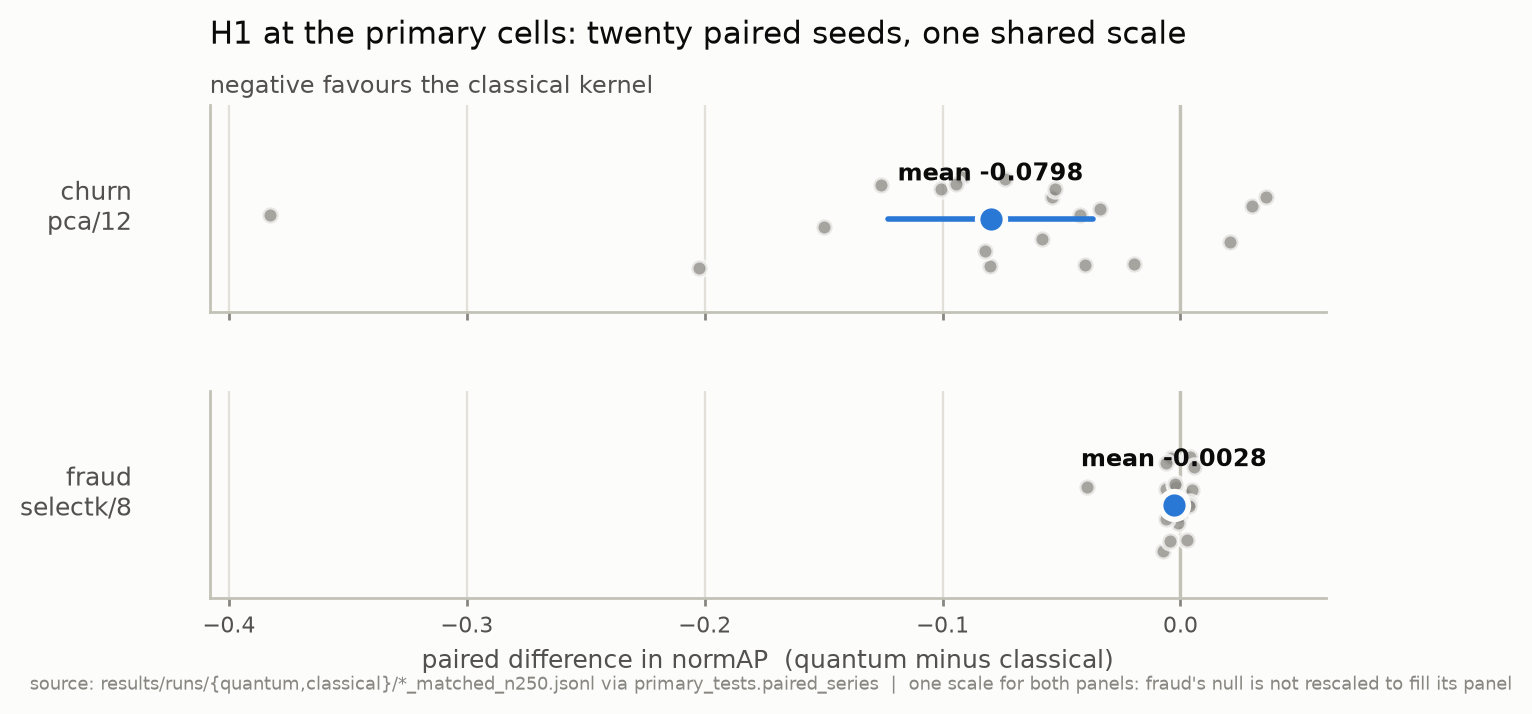
\includegraphics[keepaspectratio,alt={Figure 2 --- H1's
twenty paired per-seed differences at each primary cell, both datasets
on one shared scale.}]{fig2_h1_paired.png}}
\caption{Figure 2 --- H1's twenty paired per-seed differences at each
primary cell, both datasets on one shared scale.}
\end{figure}

\textbf{Figure 2} shows both datasets on one shared scale. Each figure
stamps its own source artefact into the image, so a reader can tell
which run it came from without trusting a caption.

\textbf{Churn, PCA at 12 qubits --- rejects, against the quantum
kernel.}

{\def\LTcaptype{none} % do not increment counter
\begin{longtable}[]{@{}lllll@{}}
\toprule\noalign{}
endpoint & mean & median & 95\% CI & Wilcoxon p \\
\midrule\noalign{}
\endhead
\bottomrule\noalign{}
\endlastfoot
normAP & -0.0798 & -0.0659 & {[}-0.1229, -0.0367{]} & 8.20e-05 \\
ROC-AUC & -0.0292 & -0.0171 & {[}-0.0457, -0.0128{]} & 3.38e-04 \\
\end{longtable}
}

Both endpoints reject and both favour the classical kernel. This is not
a failure to detect an advantage; it is a detected deficit of roughly
6.6 points of normAP at the median, in the cell chosen because it was
the classical baseline's strongest.

\textbf{The margin, stated as D6 requires.} The effect clears the
\emph{registered} MDE of 0.0171 by 4.7x and its \emph{true} primary-cell
MDE of 0.0608 by \textbf{1.31x}. The registered figure was computed from
classical-versus-classical variance and is wrong by 3.6x on this arm.
Any phrasing of the form ``well clear of what the arm was powered for''
is withdrawn.

\textbf{Fraud, SelectKBest at 8 qubits --- does not reject.}

{\def\LTcaptype{none} % do not increment counter
\begin{longtable}[]{@{}lllll@{}}
\toprule\noalign{}
endpoint & mean & median & 95\% CI & Wilcoxon p \\
\midrule\noalign{}
\endhead
\bottomrule\noalign{}
\endlastfoot
normAP & -0.0028 & -0.0014 & {[}-0.0072, +0.0017{]} & 0.245 \\
ROC-AUC & +0.0001 & +0.0005 & {[}-0.0017, +0.0019{]} & 0.823 \\
\end{longtable}
}

Reported as a bound rather than as ``no difference'':

\begin{quote}
\textbf{A true advantage larger than 0.0063 normAP at the fraud primary
cell is excluded at 80\% power.}
\end{quote}

0.0063, not the 0.0059 section 8 registered; D6 corrects it to the
primary cell's own paired sd of 0.0095. The fraud \emph{arm} as a whole
is a different quantity at 0.0138 and the two are never interchanged.
The confirmatory script printed the superseded 0.0059 for eleven days
after D6 was written, with a regression test pinning it; that is the
fifth item in \S{}5.6 and it is recorded rather than quietly corrected.

\begin{center}\rule{0.5\linewidth}{0.5pt}\end{center}

\subsection{4.3 The negative control is
clean}\label{the-negative-control-is-clean}

The full quantum pipeline on permuted labels at each primary cell, 80
records over 20 seeds.
\emph{(\texttt{results/analysis/negative\_control\_quantum.log})}

{\def\LTcaptype{none} % do not increment counter
\begin{longtable}[]{@{}lllll@{}}
\toprule\noalign{}
dataset & ROC-AUC & from 0.500 & AP vs chance & from 0 \\
\midrule\noalign{}
\endhead
\bottomrule\noalign{}
\endlastfoot
churn & 0.5058 (sd 0.0493) & +0.52 sigma & +0.0040 & +0.45 sigma \\
fraud & 0.5001 (sd 0.0452) & +0.01 sigma & -0.0008 & -0.09 sigma \\
\end{longtable}
}

Section 7's halt condition --- a consistent excess in both beyond about
two seed-level standard errors --- is not met. The comparison against
\emph{chance} AP rather than the base rate matters: the gap of +0.0154
between them is expected and is not leakage.

\begin{center}\rule{0.5\linewidth}{0.5pt}\end{center}

\subsection{4.4 H2 and H3: the prediction is not
established}\label{h2-and-h3-the-prediction-is-not-established}

\emph{(\texttt{results/audits/h2\_h3\_report.json}, 360 units, 7,200
per-seed rows)}

\begin{figure}
\centering
\pandocbounded{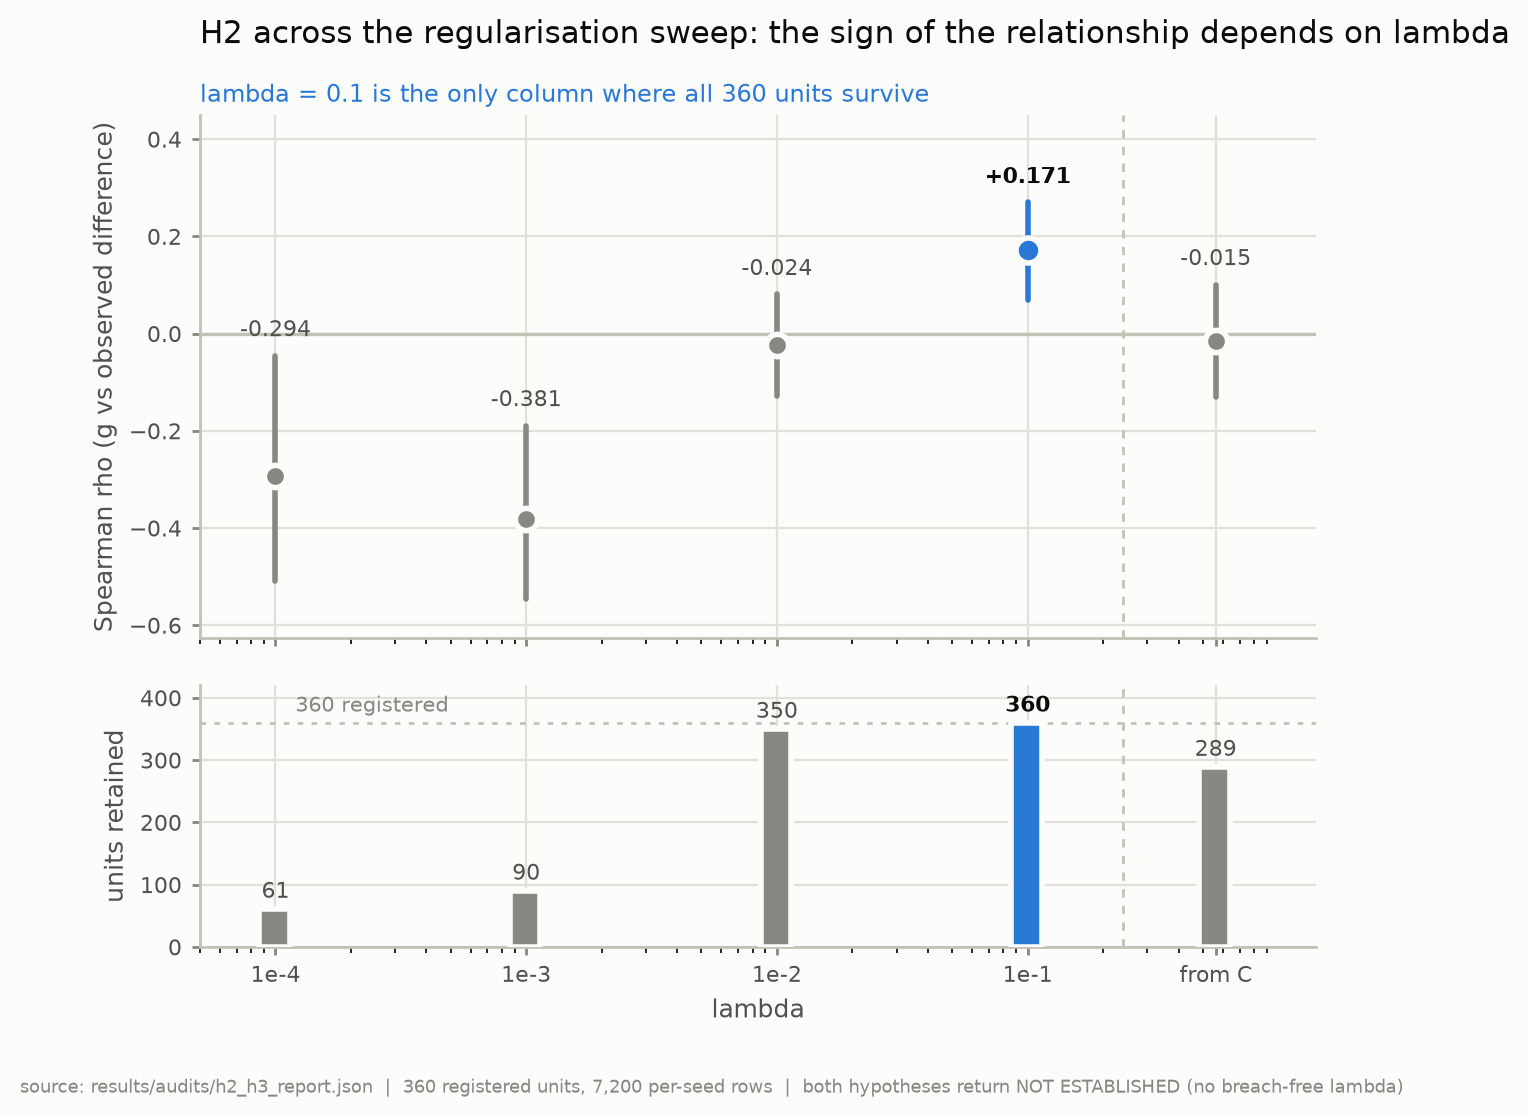
\includegraphics[keepaspectratio,alt={Figure 1 --- H2
across the frozen lambda sweep: rho with its 95\% interval above, units
retained beneath.}]{fig1_h2_lambda.png}}
\caption{Figure 1 --- H2 across the frozen lambda sweep: rho with its
95\% interval above, units retained beneath.}
\end{figure}

\textbf{Figure 1} plots this table: rho with its interval above, units
retained below, because a rho from 61 units with 299 excluded is not the
same evidence as one from all 360.

{\def\LTcaptype{none} % do not increment counter
\begin{longtable}[]{@{}
  >{\raggedright\arraybackslash}p{(\linewidth - 14\tabcolsep) * \real{0.1250}}
  >{\raggedright\arraybackslash}p{(\linewidth - 14\tabcolsep) * \real{0.1250}}
  >{\raggedright\arraybackslash}p{(\linewidth - 14\tabcolsep) * \real{0.1250}}
  >{\raggedright\arraybackslash}p{(\linewidth - 14\tabcolsep) * \real{0.1250}}
  >{\raggedright\arraybackslash}p{(\linewidth - 14\tabcolsep) * \real{0.1250}}
  >{\raggedright\arraybackslash}p{(\linewidth - 14\tabcolsep) * \real{0.1250}}
  >{\raggedright\arraybackslash}p{(\linewidth - 14\tabcolsep) * \real{0.1250}}
  >{\raggedright\arraybackslash}p{(\linewidth - 14\tabcolsep) * \real{0.1250}}@{}}
\toprule\noalign{}
\begin{minipage}[b]{\linewidth}\raggedright
lambda
\end{minipage} & \begin{minipage}[b]{\linewidth}\raggedright
units
\end{minipage} & \begin{minipage}[b]{\linewidth}\raggedright
excluded
\end{minipage} & \begin{minipage}[b]{\linewidth}\raggedright
breaches
\end{minipage} & \begin{minipage}[b]{\linewidth}\raggedright
rho
\end{minipage} & \begin{minipage}[b]{\linewidth}\raggedright
p
\end{minipage} & \begin{minipage}[b]{\linewidth}\raggedright
95\% CI
\end{minipage} & \begin{minipage}[b]{\linewidth}\raggedright
rho\(^{2}\)
\end{minipage} \\
\midrule\noalign{}
\endhead
\bottomrule\noalign{}
\endlastfoot
1e-1 & \textbf{360} & \textbf{0} & 4/7200 & +0.1712 & 1.11e-03 &
{[}+0.069, +0.270{]} & 0.0293 \\
1e-2 & 350 & 10 & 657/7200 & -0.0245 & 0.648 & {[}-0.129, +0.081{]} &
0.0006 \\
1e-3 & 90 & 270 & 4574/7200 & -0.3814 & 2.09e-04 & {[}-0.545, -0.189{]}
& 0.1454 \\
1e-4 & 61 & 299 & 4972/7200 & -0.2938 & 2.16e-02 & {[}-0.508, -0.045{]}
& 0.0863 \\
from C \(\dagger\) & 289 & 71 & 2893/7200 & -0.0145 & 0.806 & {[}-0.130,
+0.101{]} & 0.0002 \\
\end{longtable}
}

\textbf{\(\dagger\) The \texttt{from\ C} row was computed under the
\(\lambda\) rule D14 has since withdrawn}, 1/(2\(\cdot\)C\(\cdot\)n).
Under the adopted 1/(2C) that column's ceiling breaches fall from
\textbf{2,893 to 979 of 7,200}, which still leaves it not breach-free.
Its rho was \textbf{not} recomputed: the verdict does not turn on it,
and D14's outcome-to-verdict mapping authorised reading the breach
status and nothing further. The row stands as the figure the published
verdict was computed from, labelled, rather than being silently replaced
by a number computed after the fact.

\textbf{Both return
\texttt{NOT\ ESTABLISHED\ (no\ breach-free\ lambda)}.} D5 requires the
conclusion to hold at every lambda at which no unit breaches its sqrt(n)
ceiling, and no column is breach-free.

\textbf{What that verdict is, said precisely, because three different
statements are easy to confuse here.} The registered rule returned
\textbf{no verdict}. That is not the same as the prediction having been
tested and failed, and it is not the same as finding no relationship. At
lambda = 0.1 the null \textbf{is} rejected, in the direction Huang
predicts. The registered rule declined to speak because its precondition
--- a column in which no unit breaches its ceiling --- is met by none of
the columns.

Three things a reader needs in order to weigh that.

\textbf{It turns on four rows.} At lambda = 0.1 the column is otherwise
complete --- all 360 units present, none excluded --- and fails by
\textbf{four breaching seeds out of 7,200}, 0.056\% of the observations,
all from one cell and seed (churn, n=100, selectk, 4 qubits, seed 7).
The next-largest g/ceiling ratio anywhere is 0.9150 against those four
at 1.075 to 1.093, so the dependence is discontinuous rather than
marginal. No tolerance was introduced and no seed excluded.

\textbf{The permissive reading also fails.} D5's text admits a second
reading under which the rule reduces to agreement across all five
columns. That fails too, because the sign of rho reverses: +0.17 at
lambda = 0.1 against -0.38 at 1e-3 and -0.29 at 1e-4. Both readings land
on the outcome D5 pre-declared for disagreement: g's relationship to
observed performance depends on the regularisation chosen, which is a
result about the metric.

\textbf{The substantive number is rho\(^{2}\), not the verdict.} At
lambda = 0.1, the only column with a complete unselected population,
\textbf{rho\(^{2}\) = 0.0293}: the geometric difference accounts for
under three percent of the rank variance in observed difference. A
quantity explaining three percent of rank variance, whose sign moves
with a parameter the practitioner chooses, cannot tell a practitioner
not to bother. That is a claim about \textbf{usability}, not about
absence, and it is the finding the registered design called the
practically valuable outcome to establish either way.

\textbf{A third \(\lambda\) rule was evaluated and returned nothing to
test.} Huang's own g\_tra selection over his declared grid was specified
in advance (D16) and run. It does not select a \(\lambda\) at all on
76.5\% of the units, so it yields an incomplete column and is reported
as \textbf{unresolved} rather than as a negative result. \S{}6.2a gives
the measurement. Counting it, three \(\lambda\) rules have been
evaluated and none produces a breach-free column; the third produces no
column.

\textbf{H3 carries two readings and the reader picks.} Section 9
registers H3 as subordinate to H2 and reported only if H2 is rejected.
It was ungated in week 4, for a stated and good reason, and the
departure was not recorded until 29 September --- after H3's result had
been computed and published. A reader who accepts the commit ordering
may read H3 as confirmatory under a departure declared late but decided
early; a reader who does not should read it as exploratory. The paper
does not choose for them.

\begin{center}\rule{0.5\linewidth}{0.5pt}\end{center}

\subsection{4.5 The exploratory
families}\label{the-exploratory-families}

Exploratory throughout, Holm-corrected within each family, and no
finding here bears on H1 or H2. Each tested level averages the cells at
that level \textbf{within each seed} before testing, because cells at
one seed share a train/test split; levels carry 20 paired observations,
not pooled rows.
\emph{(\texttt{results/analysis/exploratory\_sweep.json},
\texttt{results/analysis/primary\_tests.json})}

\begin{figure}
\centering
\pandocbounded{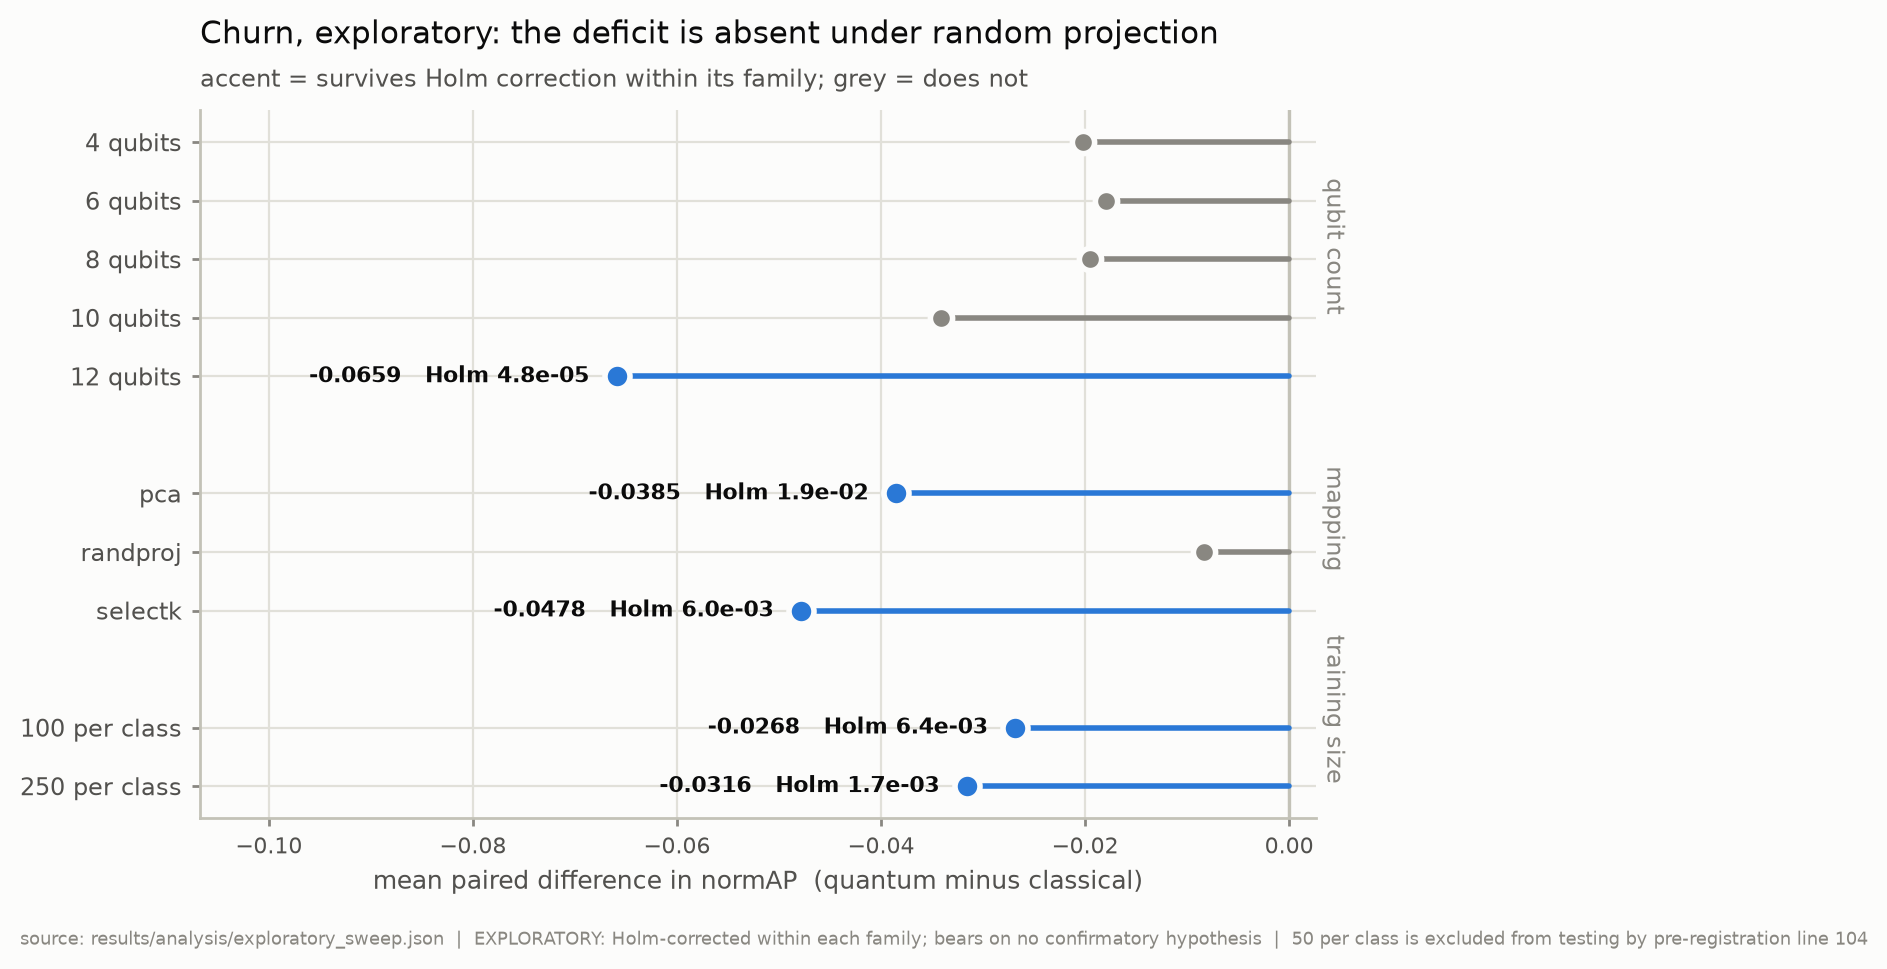
\includegraphics[keepaspectratio,alt={Figure 3 --- the
churn exploratory families, with Holm-significant levels in the accent
colour.}]{fig3_churn_exploratory.png}}
\caption{Figure 3 --- the churn exploratory families, with
Holm-significant levels in the accent colour.}
\end{figure}

\textbf{Figure 3} shows the churn families.

\textbf{Churn.} The deficit survives correction under PCA (-0.0385, Holm
0.0189) and SelectKBest (-0.0478, Holm 0.0060) and \textbf{not} under
random projection (-0.0084, Holm 0.3884). It survives at both tested
training sizes (-0.0268 at 100, -0.0316 at 250; the 50-per-class arm is
registered as not for hypothesis testing and is reported descriptively
at -0.0315). In the qubit family only 12 survives (-0.0659, Holm
4.77e-05).

Per setting against the best classical kernel, all four lose after
correction: angle-r1 -0.0606 (Holm 0.0017), angle-r2 -0.0959 (5.34e-05),
iqp-r1 -0.1011 (7.63e-06), iqp-r2 -0.3008 (7.63e-06). \textbf{The
headline does not depend on the quantum side being allowed to choose},
which is what section 9 required this second reporting mode to show.

Across all 15 cells, two survive Holm: pca/12 at -0.0798 (Holm 0.0012)
and selectk/12 at -0.0918 (0.0082).

\textbf{Fraud.} Nothing survives anywhere. Largest magnitude +0.0045, no
Holm-adjusted p below 0.19. Three figures are \textbf{below D2's 1e-3
precision floor and are reported as below the pipeline's resolution
rather than as measurements}: qubit 10 at -0.0008, random projection at
+0.0003, training size 250 at -0.0000.

\textbf{Provenance of the per-setting and all-cells families.} Until 6
October both were printed and never returned, so the only trace of them
was three rounded values per level in a tracked log, with no n, median,
sd, confidence interval or sensitivity t-test, and no commit, input
digest or seed list. They are now persisted with all of those. The
figures above are unchanged: stdout was byte-identical across that
change on all six arms.

\begin{center}\rule{0.5\linewidth}{0.5pt}\end{center}

\subsection{4.6 What these numbers do not
support}\label{what-these-numbers-do-not-support}

Stated explicitly because each was reachable and each would have been
wrong.

\textbf{No trend with qubit count.} The cell-level trend on churn is rho
= -0.4692, p = 0.0777 on n = 15 cells --- not significant. Only the
12-qubit level survives Holm. ``The deficit deepens with qubit count''
is not supported, and the unit of analysis here is the cell: an earlier
version of a trend statistic in this project correlated 300 records
instead of 15 cells and every figure it printed was voided.

\textbf{No claim about fraud's ROC figures against the AP floor.} D2's
floor is 1e-3 \emph{in average precision}. Fraud's ROC-AUC mean of
+0.0001 is numerically smaller but on a different scale, and flagging it
would repeat the unit conflation D6 records.

\textbf{No claim that g carries no signal.} At lambda = 0.1 the
relationship is statistically detectable and in the predicted direction.
The claim in \S{}4.4 is that it is not usable as a screen at that effect
size with that sign instability, which is a different and narrower
statement.

\textbf{One structural reading, offered as interpretation.} On churn the
deficit is absent exactly where the classical baseline is weakest:
random projection is the mapping week 3 measured as climbing most with
dimension, 0.3678 to 0.5481, and it is the one mapping where the quantum
kernel is not significantly behind. If that holds up it inverts the
usual framing, since the regime of interest is supposed to be the one
where classical methods already do well. It rests on one dataset and one
non-significant contrast.

\begin{center}\rule{0.5\linewidth}{0.5pt}\end{center}

\subsection{4.7 Limitations, including two this study
created}\label{limitations-including-two-this-study-created}

\textbf{The artefact was not available, and this conditions every
limitation below it.} The repository was \textbf{private from 17
September to 15 October 2026}, the whole of the project's working life.
It was found on 15 October, when a Software Heritage save request failed
with \texttt{visit\_status:\ not\_found} and an unauthenticated GitHub
query returned 404; the author's pushes had always succeeded because the
author is authenticated. \textbf{No reader could have checked any claim
in this study while it was being made.}

The consequence for ordering is the one that matters. D14 required its
chosen option and outcome-to-verdict mapping to be ``committed and
pushed before any recomputed value is examined'', and D16 was
``specified in full and pushed before it was computed''. Both happened.
\textbf{Neither was public.} A push to a private remote does leave
server-side receipt times the author does not set, which a purely local
commit does not, but those times are not exposed to a reader, not
verifiable by one and not citable. So every phrasing of the form
\emph{declared publicly} or \emph{published before the run} is
\textbf{withdrawn} in favour of \emph{committed and pushed to a private
remote before}, and the pre-commitment discipline here is something the
author practised rather than something a reader can check.

\textbf{Visibility was changed on 15 October 2026}, after two Software
Heritage save requests (2558108, 2558127) had failed with
\texttt{visit\_status:\ not\_found} against the private origin. A third
request succeeded at \textbf{01:33:06 UTC on 15 October 2026},
\texttt{visit\_status:\ full}. A fourth was taken three minutes later.
\textbf{There are two snapshots and the reason is structural:}

\begin{verbatim}
swh:1:snp:bdbf43089b1ed77f5ec9307e11f5c255dddc84dd   01:33:06, repository at 5464088
swh:1:snp:c19a29f94639c2ea87347ae40a3d949919a75005   01:36:58, includes the commit recording the first
\end{verbatim}

\textbf{A snapshot cannot contain its own citation.} The first attests
the repository as it stood when visibility changed, before any record of
the archive existed; a reader resolving it finds a \S{}4.7 that does not
mention it. The second contains the commit that records the first, so it
is the one to resolve to read this paragraph as archived. The second is
in turn cited by a commit made after it, and \textbf{that regress does
not terminate} --- it is stopped here by choosing to stop, not by
completeness, and the same is true of any self-referential archive
citation.

\textbf{These are the first externally verifiable facts in this study.}
A third party now attests that this repository's content existed in that
exact form at or before that instant, at a time no one here controls.
Everything below describes what a reader can do from that moment on.

\textbf{What the snapshot does not do}, stated because an archive
identifier invites being read as more than it is. It \textbf{backdates
nothing}: every result, every deviation record and every pre-commitment
in this paper predates it and remains externally unattested. It does
\textbf{not} repair D11, and could not: both snapshots capture the
public refs as they stood on 15 October, six days before
\texttt{prerewrite-20260925} was published, so neither archive contains
the commits the result records name. Those identifiers resolve from the
repository itself and not from the archive. What the snapshots establish
is forward-looking only: from 01:33 on 15 October 2026, a claim about
this repository's state can point at something outside this machine.

\textbf{Provenance, and the decision that was open until 21 October
2026.} Every one of the 15,120 result records stores a
\texttt{git\_commit} that a history rewrite on 25 September 2026 removed
from the public repository. The recovered branch
\texttt{prerewrite-20260925} was \textbf{published on 21 October 2026},
tip \texttt{b5bf0431}, and all five identifiers this study depends on
are reachable from it: \texttt{a8bafbb} and \texttt{61f7db9}, which
\texttt{pre-registration.md} cites as its anchor, and \texttt{0b796a3},
\texttt{2cf7ec7} and \texttt{0b2aef4}, which the records store.
\textbf{A reader can now compute the tree of a stored hash directly.}
The annotated tags \texttt{records-0b796a3}, \texttt{records-2cf7ec7}
and \texttt{records-0b2aef4} remain as a convenience and are no longer
the only route; a tag records an assertion, and the assertion is now
checkable against the object it is about.

\textbf{What that closes and what it leaves.} It closes the binding: a
record names a commit, the commit is public, its tree can be computed by
anyone. It closes nothing about \textbf{ordering}. Commit dates are
author-set, both histories are author-controlled, and the two Software
Heritage snapshots were taken six days before this branch was public, so
neither contains it. A re-run from current HEAD still produces evidence
about the current code rather than authenticating the old records. The
limitation that remains is the one in the next paragraph, and it is the
one that was always the larger of the two.

\textbf{The cost, stated rather than minimised.} Publishing restored to
the public repository the AI co-authorship trailers the rewrite removed,
across the branch's 25 commits. \texttt{main} already carried
\textbf{twenty} commits with those trailers, reinstated by default in
late September and then deliberately left in place and documented rather
than rewritten, and this repository's README declares the assistance in
prose. The decision therefore conceded in public what the record had
already conceded four weeks earlier. It is recorded as an amendment to
D11.

\textbf{No external timestamp, and no external reader either.} This
study is not registered at OSF and has \textbf{no Software Heritage
snapshot predating its results}. The first of those is a
\textbf{decision} rather than an omission, taken on 21 October 2026 and
recorded against D11: a registration created now would be dated three
weeks after every result and after this paper was written, and attaching
it to a document whose header once claimed an earlier date would read as
backdating, converting an honest absence into an apparent
misrepresentation. Two weekly reports had listed it as outstanding work
without reconciling that against the reasoning already in D11.

Its ordering evidence is an author-controlled history, rewritten once on
25 September, on a remote that no one else could read until 15 October,
with no external attestation at any point. Every ordering claim in this
paper, including the claims in D13, D14 and D16 that a decision preceded
a result, rests on evidence of that class. \textbf{A reader who declines
to accept it is left with nothing}, and that is the honest statement of
the position rather than a reason to discount the claims selectively.

\textbf{No hardware.} The IBM runs registered for weeks 7 to 8 were
dropped as infeasible (D12) and no claim in this paper depends on them.

\textbf{The 50-per-class arm} resolves 0.1368, three times coarser than
the 0.0427 that already disqualified it from hypothesis testing.

\textbf{One dataset is saturated.} Fraud's classical baseline sits at
0.9659 normAP at the primary cell and is saturated at every training
size tested, so one of the two datasets could not have shown an
advantage had one existed.

\textbf{The figures, and a reversed decision.} The three PNGs above are
\textbf{committed}, by name, as exceptions to the \texttt{.gitignore}
rule that excludes \texttt{results/figures/*}. An earlier draft excluded
them on the ground that outputs are regenerated rather than versioned
and that \texttt{PYTHONPATH=src\ python\ scripts/make\_figures.py}
reproduces them deterministically from committed artefacts. That
reasoning is sound as far as it goes and the regeneration command still
works. It was reversed for one reason it did not address:
\textbf{determinism there rests on an unpinned plotting library}, so a
reader on a different matplotlib gets a visually different figure, and a
figure a paper references but does not ship is the same defect class as
a commit hash that does not resolve. Three PNGs are 319 KB. The SVG
sources remain excluded, being regenerable and read by nothing in the
paper.

\textbf{Checks this study has not completed}, listed rather than left
implicit.

\textbf{The mutation harness now reads every test file, and what it
reveals is worse than what it fixed.} Until 15 October it was hardwired
to one test file, so mutants for the F20 diagnostic, the \(\lambda\)
correction and the exploratory families had to be run by hand. Those
four are now in the suite and all \textbf{37} mutants are killed by the
test that names each one, across five source files and four test files.
But the coverage report was also scanning only the files that already
had mutants, which hid every file with none: corrected, it reads
\textbf{37 of 395 test functions}, not the 34 of 70 the old report
implied. \textbf{Fifteen of nineteen test files have no mutant at all},
including \texttt{tests/test\_audit.py} and its 76 functions --- the
tests for the audit tool \S{}5 is about. So the honest statement is that
this project has demonstrated non-vacuity for 9\% of its test functions
and has not examined the rest.

\textbf{The one check that had no mutant now has two.}
\texttt{select\_lambda} in \texttt{scripts/gtra\_sweep.py}, which
implements D16's selection rule, was exercised only by that script's own
control F and not by pytest. The harness maps each mutant to a pytest
node, so a rule with no pytest test cannot have its non-vacuity
demonstrated at all, and control F runs inside a sweep that takes hours.
\texttt{tests/test\_gtra\_sweep.py} now pins the rule, and two mutants
target it: taking the smallest admissible \(\lambda\) rather than the
largest, and reading the threshold as strict where D16 fixed it
inclusive. Both are killed. One of those tests covers a case control F
does not --- an admissible set with a hole in it, where an
implementation scanning upward for the first violation would agree with
control F on every monotone input and still select the wrong
\(\lambda\).

\textbf{The figures check covers three of this paper's numbers.}
\texttt{scripts/check\_paper\_figures.py} re-derives the churn and fraud
primary-cell exclusion bounds from
\texttt{results/audits/d6\_table.json}, and D16's share of units with no
admissible \(\lambda\) from the 7,200 stored unit records, comparing
each at the precision this paper states rather than within a chosen
tolerance. Everything else it reports as \textbf{not checked}, against a
denominator of every decimal figure in this paper, which it counts on
each run rather than quoting from here so that the figure cannot go
stale the way this section's own items did. The denominator is left
unfiltered on purpose: it includes section cross-references, arXiv
numbers and DOIs that are not measurements, and filtering those by
pattern would be a guess, which is what made the mutation coverage above
overstate itself. Among the figures it does \textbf{not} cover are the
H2 rank correlation and D16's elasticities, whose quantities have not
been mapped to an accessor in any stored record. \S{}5.6 records that
this check would not have caught any of the defects that motivated it.

\textbf{One item unchanged, and two closed since.} \textbf{Two Software
Heritage snapshots now exist},
\texttt{\seqsplit{swh:1:snp:bdbf43089b1ed77f5ec9307e11f5c255dddc84dd}} at 01:33:06
and \texttt{\seqsplit{swh:1:snp:c19a29f94639c2ea87347ae40a3d949919a75005}} at
01:36:58 UTC on 15 October 2026, after two earlier requests failed
against the private origin. It postdates every result here, so it bounds
the provenance gap rather than closing it; the first paragraph of this
section states what it does and does not establish.

The other two are closed, and one of them was described wrongly here.
The \texttt{descriptive\_only} rows in the exploratory output now carry
the \texttt{below\_d2\_floor} field the tested rows carry. The grid
adequacy check was said to have ``not been extended since week 9'',
which misplaced the gap: the measurement was complete and correct in
week 3 and reproduces bit-identically under current code, and what was
missing was that its adjudication lived only in prose.
\texttt{scripts/check\_grid\_edges.py} went on printing the rule week 3
had withdrawn, reporting UNDER-TUNED on fraud where the registered
comparison against a shuffled-label null returns adequate on both
datasets. The registered comparison is now what the script computes and
what its output records; \S{}5.6 counts the episode.

\begin{center}\rule{0.5\linewidth}{0.5pt}\end{center}

\section{Section 5 --- The protocol}\label{section-5-the-protocol}

\textbf{Draft, 4 October 2026.} Written under the framing recorded in
D15, which makes this section the paper's contribution rather than its
methods appendix.

A comparison of quantum and classical kernels can be run carefully and
still mean nothing, because the ways it fails are not visible in its
results. This section specifies checks that are, says what each costs,
and is explicit about which of them is implemented tooling and which is
a procedure performed by hand.

It audits \textbf{method, not results}. It never reports which model
won. A failure means a conclusion drawn from a file is not supported
\emph{by that file}; it does not mean the conclusion is wrong.

\begin{center}\rule{0.5\linewidth}{0.5pt}\end{center}

\subsection{5.1 Three parts, and only one of them is a
tool}\label{three-parts-and-only-one-of-them-is-a-tool}

D15 describes this project's contribution as a process for checking
equation ordering, implementation fidelity, provenance, and the limits
of the resulting evidence. \textbf{The implemented protocol covers the
fourth and part of the second.} Saying so first is the point; a section
that let the framing imply more tooling than exists would be the error
the protocol is for.

{\def\LTcaptype{none} % do not increment counter
\begin{longtable}[]{@{}
  >{\raggedright\arraybackslash}p{(\linewidth - 6\tabcolsep) * \real{0.2500}}
  >{\raggedright\arraybackslash}p{(\linewidth - 6\tabcolsep) * \real{0.2500}}
  >{\raggedright\arraybackslash}p{(\linewidth - 6\tabcolsep) * \real{0.2500}}
  >{\raggedright\arraybackslash}p{(\linewidth - 6\tabcolsep) * \real{0.2500}}@{}}
\toprule\noalign{}
\begin{minipage}[b]{\linewidth}\raggedright
part
\end{minipage} & \begin{minipage}[b]{\linewidth}\raggedright
what it checks
\end{minipage} & \begin{minipage}[b]{\linewidth}\raggedright
status
\end{minipage} & \begin{minipage}[b]{\linewidth}\raggedright
exercised on
\end{minipage} \\
\midrule\noalign{}
\endhead
\bottomrule\noalign{}
\endlastfoot
\textbf{A. The record audit} & what a results file does and does not
support & \textbf{implemented}: \texttt{scripts/audit.py},
\texttt{tests/test\_audit.py}, a documented record format and a hook
interface & this project's six arms; one foreign pipeline \\
\textbf{B. Source to implementation} & that a paper's printed equation,
its stated interpretation, and its released code are the same thing &
\textbf{procedure, not tooling}. No script. & two published papers \\
\textbf{C. Provenance} & that a result's stated origin can be resolved
by a reader & \textbf{procedure, not tooling}. No script. & this
project, against itself \\
\end{longtable}
}

Parts B and C are written up here because they found things, and because
a reader deciding whether to repeat them deserves the cost. They are not
claimed as software.

\begin{center}\rule{0.5\linewidth}{0.5pt}\end{center}

\subsection{5.2 Part A --- the record
audit}\label{part-a-the-record-audit}

\subsubsection{The format}\label{the-format}

One JSON object per line; a record is one model, scored once, on one
train/test split. Nothing in it is specific to quantum kernels.
Required: \texttt{method}, \texttt{seed}, \texttt{n\_train},
\texttt{n\_test}, \texttt{test\_base\_rate},
\texttt{test\_average\_precision}, \texttt{test\_roc\_auc}. Strongly
recommended, with each check degrading to SKIP and naming what its
absence makes unanswerable: \texttt{test\_label\_fingerprint} (the test
labels hashed \textbf{in order}, without which no paired test can be
verified, only assumed), \texttt{shuffled}, \texttt{final\_converged},
\texttt{inner\_score}.

The format is the load-bearing part. \textbf{A file that does not record
enough to be checked cannot be checked by anyone}, and the claim here is
not that a comparison lacking these checks is wrong --- it is that
nobody, including its authors, can tell.

\subsubsection{What it asserts, and what it
costs}\label{what-it-asserts-and-what-it-costs}

Tier 1 runs from the records file alone: schema, chance correction,
negative control, pairing integrity, solver health, unit of analysis,
statistical power, precision floor, multiplicity, tuning symmetry,
cross-arm comparison, selection. \textbf{Cost: seconds, no access to the
original pipeline.} This is the tier that makes auditing a stranger's
comparison cheap.

Tier 2 asks about the kernel, which a results file does not contain, so
the pipeline supplies three optional functions --- \texttt{gram},
\texttt{training\_data}, \texttt{refit} --- and the audit imports
nothing of its own. It covers kernel conditioning and classical
surrogate equivalence. \textbf{Cost: kernel recomputation, which is the
dominant expense}; \texttt{-\/-hook-sample} is the knob, and readings
are indicative by construction. They say \emph{run the full analysis},
not \emph{publish this}.

One check needs a re-run rather than a hook: \textbf{grid adequacy
against a shuffled null}, because widening a grid raises the best inner
score even when nothing is better, so hyperparameter edge flags never
justify it on their own. \textbf{Cost: a second full execution of the
pipeline on permuted labels.} It is the most expensive check here and
the one most often skipped.

\subsubsection{What distinguishes these from
diagnostics}\label{what-distinguishes-these-from-diagnostics}

Published work in this area is statistically careful. Kakavand et
al.~apply paired Wilcoxon with an exact permutation fallback for small
n, Friedman with post-hoc Nemenyi, and both Benjamini-Hochberg and
Bonferroni; their kernel diagnostics compute condition number, effective
rank, PSD-ness and the full eigenspectrum; their preprocessing is
leakage-safe and their two arms share one hyperparameter grid --- a
symmetry this project's registered design did not have. \textbf{That is
more statistical care than this project had at the end of week 4}, and
the protocol does not claim otherwise.

What is added are \textbf{decision rules rather than diagnostics}: a
measured reproducibility floor below which a difference is reported as
unresolvable rather than small; classical surrogate equivalence
expressed in endpoint units rather than as a distance in kernel space;
shuffled-label controls adjudicated against both a sigma bar and that
floor; cross-arm rather than within-arm power, which differ by 2.3x to
3.9x in this project's own data. Computing a condition number is
ordinary. Refusing a verdict on the strength of one is not.

\begin{center}\rule{0.5\linewidth}{0.5pt}\end{center}

\subsection{5.3 Part B --- source to
implementation}\label{part-b-source-to-implementation}

\textbf{No tooling exists for this.} It is a reading procedure,
performed twice, and it found something both times.

\textbf{The procedure.} Obtain the paper's source rather than a
rendering --- for arXiv, the e-print LaTeX. Record the archive and file
hashes. Locate the equation as printed, with its subscripts. Locate the
prose that assigns its arguments. Locate the corresponding call in the
released code. Then compare the three, and label every resulting
statement as what the source states, what the implementation does, or
what the comparison establishes.

\textbf{Why source rather than a rendering.} Earlier attempts in this
project to read Huang's Appendix F from PDF renderings returned
transcriptions that were internally contradictory on exactly the
subscripts at issue, and a claim that the appendix contradicted its own
main text was drafted on that basis and withdrawn when the LaTeX was
read. \textbf{A claim about an equation's index placement is worth no
more than the characters it was read from.}

\textbf{Cost.} One download, the hashes, and an afternoon per paper. No
compute. It is the cheapest part of this protocol and it caught the
largest thing.

\textbf{What it found} is in section 2: that Huang's F19 is the reversed
ordered comparison relative to Equation (5), that Flórez Ablan et
al.~read it the natural way, and that the quantity they compare against
\(\sqrt{N}\) is therefore \texttt{g(K\_Q\textbar{}\textbar{}K\_C)} where
the screening quantity is \texttt{g(K\_C\textbar{}\textbar{}K\_Q)}. It
also found, in their released code, ROC-AUC computed on hard predicted
labels --- making the reported quantity balanced accuracy rather than a
ranking measure --- and \texttt{g\_tra} computed throughout and never
compared to anything.

\textbf{What it does not establish.} Nothing about whether their
conclusions are wrong. An ambiguity inherited from an upstream appendix
is a scope statement, not an error attributed to the people who
inherited it.

\begin{center}\rule{0.5\linewidth}{0.5pt}\end{center}

\subsection{5.4 Part C --- provenance}\label{part-c-provenance}

\textbf{No tooling exists for this either.} The procedure is: take the
identifier a result record stores for its own origin and try to resolve
it as a stranger would, from the public artefact alone.

\textbf{Cost.} Minutes, and it requires no access to anything the
authors have not already published --- which is the point.

\textbf{What it found, run against this project.} Every one of the
15,120 result records stores a \texttt{git\_commit} that does not exist
on the public repository. A history rewrite invalidated all three stored
hashes; they resolve only from a branch recovered from a folder that had
been queued for deletion. A tree-identity mapping to public counterparts
exists, and it reduces what must be taken on the author's word without
removing it: a reader can verify that the counterpart carries the stated
tree and cannot verify that the stored hash ever did.

The project's own reproducibility section commits that every record
stores its commit. \textbf{That commitment was satisfied in form and
unverifiable in practice for nine days before anyone checked}, and it
was checked only because a previous amendment had documented the same
trap for different hashes.

\textbf{The loss, bounded precisely.} What a reader cannot do is
\textbf{independently bind a historical result record to the code that
generated it}. That is the whole of it, and it is not nothing: they
cannot confirm that the analysis code at run time is the code now
published, nor diff the two to see what differs.

\textbf{What remains independently checkable}: every analysis script, in
full; the data provenance, which is separate and unaffected, with
sources and checksums in \texttt{data/README.md}; the records
themselves, which are intact; and the public half of the tree-identity
mapping --- that each named counterpart on \texttt{main} carries the
stated tree.

\textbf{What a re-run does not do.} Executing the current pipeline on
the current data produces \textbf{new evidence about the current code}.
It does not authenticate the old records, because agreement would be
consistent with the code having changed in ways that do not alter these
particular outputs, and disagreement would not distinguish a code change
from a data or environment change. A reproduction and an authentication
are different operations, and only the first is available here.

\begin{center}\rule{0.5\linewidth}{0.5pt}\end{center}

\subsection{5.5 What this protocol does not
do}\label{what-this-protocol-does-not-do}

It does not tell you whether a quantum kernel is better. The hook widens
what it can see and does not change that: a surrogate reading is about
the kernel, never about which model won. It does not detect a wrong
kernel implementation, a mis-specified feature map, or a dataset leaking
labels through preprocessing. It cannot see analysis performed outside
the file it is given. \textbf{A clean report means the file supports the
kind of claim being made, not that the claim is true.}

Parts B and C are not automatable as written. Part B requires judgement
about what an equation means; part C requires knowing what a given
repository's history has been through.

\begin{center}\rule{0.5\linewidth}{0.5pt}\end{center}

\subsection{5.6 The evidence for this protocol is weaker than its
instance count
suggests}\label{the-evidence-for-this-protocol-is-weaker-than-its-instance-count-suggests}

This is the section a reader should weigh most heavily, and it argues
against the contribution.

\textbf{Every Tier 1 and Tier 2 check was written after the defect it
catches.} The protocol's own first section says so: each exists because
a specific reading went wrong here, usually after passing review.
Seventeen deviation records and a list of caught mistakes are
\textbf{not} evidence that a tool catches a stranger's mistakes. They
are evidence that this project eventually noticed its own.

\textbf{The prospective evidence is one case, and what it shows needs
stating precisely.} In week 6 the audit was run against Kakavand et
al.'s public Zenodo deposit through an adapter. It produced \textbf{one
measurement and eight refusals}: kernel conditioning across all six
deposited \texttt{ibm\_fez} Grams, worst 4.5e+05, against this project's
own 7.8e+19 to 1.1e+33; and eight statements of what the deposit cannot
answer --- four required fields absent, so chance correction, power and
the precision floor each name their gap; no classical arm in the
hardware phase, so cross-arm has nothing to pair; one seed, so
unit-of-analysis warns and power cannot speak; no \texttt{inner\_score},
so selection cannot be shown.

\textbf{It found no defect in their pipeline, and was not looking for
one.} The week-6 record states it directly: \emph{``None of this is a
criticism of their work: it is a map of what a reader can and cannot
verify from that deposit.''}

\textbf{The criterion by which this counts as useful, stated rather than
assumed.} The output is useful if it changes what a reader knows about
the deposit's evidential reach. Before the run, a reader could not say
which questions those records could answer; after it, they could, in
seconds, without the originating pipeline. That criterion is met.
\textbf{It is a claim about a reader's state of knowledge, not about the
quality of the audited work}, and it does not generalise to defect
detection, because on the only occasion these checks met foreign records
they detected none.

Parts B and C add two cases apiece, but both were performed by the same
party that wrote the procedures.

\textbf{Seven things have gone wrong in public, and they are two
different kinds.} Collapsing them under one word was itself imprecise.

\emph{Defects in the instrument (three).} On its first contact with real
records the tool required a field this project's own pipeline never
emitted, collapsed fifteen configurations into one, and \textbf{silently
changed three answers}. The first audit run against real records then
found four further defects, \textbf{all four in the checks rather than
in the records}, with the full test suite passing on every one.

The third is the registered adjudicator of grid adequacy. Section 7 of
the pre-registration names \texttt{scripts/check\_grid\_edges.py} as
what decides whether a grid is too narrow, and requires the decision to
be made against a shuffled-label null. The script computed that null
when asked, printed it, and told the reader to do the subtraction by
hand, while on a real run printing a verdict derived from the ratio of
the gain to the minimum detectable effect. Week 3 had already recorded
that ratio as a defect, because the maximum over a grid grows with the
number of points searched and so cannot separate an optimum lying
outside the grid from a surface too noisy to rank; the threshold week 3
describes as pre-declared existed nowhere in the code. The committed log
\texttt{results/analysis/grid\_edges\_fraud.log} therefore carried the
verdict \textbf{UNDER-TUNED, widen the grids and re-run week 3}, where
the registered comparison returns adequate. The correct answer was in
the week-3 record throughout and the project acted on it, so no result
here rests on the wrong verdict; what was published was an instrument
contradicting its own record for three weeks. Found on 18 October 2026
by reading the script, not by any check in this protocol.

\emph{Claims its authors made that their own data does not support
(four).} It asserted from the manuscripts that two published benchmarks
performed none of five checks; when the deposit behind one was read,
\textbf{six of seven claims in that paragraph were wrong or misleading}.
It declared four checks unrunnable when three were not --- one needed
nothing at all. And the confirmatory script printed a \textbf{superseded
exclusion bound for eleven days}: \texttt{scripts/primary\_tests.py}
quoted the registered 0.0059 for fraud's primary cell while every
document here quoted D6's corrected 0.0063, the committed analysis log
carried the wrong figure, and a regression test asserted it. Nobody
re-read the code after writing the correction. It was found on 6 October
2026 while refactoring an unrelated function, by inspection and not by
any check in this protocol. And the pre-registration gives the measured
advantage of extending a grid on random labels over real ones as
\textbf{five to seven times}, which is the polynomial-kernel figure: on
the RBF kernels the ratio is 2.0 and 35.7, so two of the four
measurements fall outside the stated range, one above it and one below.
Week 3 had the full four-row table in front of it when that sentence was
written. \textbf{This fourth one differs in kind from the three before
it}, and the difference does not favour it: those asserted things nobody
had checked, while this took a measurement that had been made correctly
and stated it more broadly than it supported. Nothing in a reader's view
distinguishes a generalised measurement from a measured one. The rule
that figure supports is unaffected, the direction holding on every
kernel and both datasets; D17 records it and the registered document is
not edited.

\textbf{None of the seven is an audited pipeline failing an audit.} A
reader who takes this section as evidence that audited work fails these
checks has read it as it was first written and not as it is meant. The
two kinds matter differently: the first says the instrument needed
repair, the second says its authors committed the error the instrument
exists to prevent.

\textbf{A further item, about Tier 2 rather than about either kind.} On
a partial sample of two of the six foreign Grams, the conditioning check
read 1.7e+04 --- \textbf{understating the worst case by a factor of 26}.
Two things should be kept apart here. The numerical miss was corrected
only by running the full six. What printing the sample count achieved
was narrower: it exposed that coverage was incomplete, so the reading
was known to be partial. \textbf{It did not establish the true worst
case and could not have.} That is the honest limit of indicative
sampling, and it argues for treating \texttt{-\/-hook-sample} readings
as a prompt to run the full analysis rather than as a figure.

\textbf{A bounded gap the fifth item exposes, and two more beside it.}
The superseded bound was found by inspection, not by a check. So were
two latent defects in this project's own reporting code, found the same
day: a Holm family size printed as the literal 4 rather than computed,
and a table headed ``all cells'' that silently skipped cells with too
few paired series. Neither of those two ever produced a wrong value, so
neither joins the count above; the superseded bound did, so it does. The
sixth item above, the grid adjudicator, was found the same way. What all
four share is the route. \textbf{Tier 1 reads records and Tier 2 reads
kernels. Nothing in this protocol reads this project's own analysis and
reporting code for claims the data does not support}, which is where all
four lived.

\textbf{What now exists, and what it would not have caught.} Since 19
October 2026 \texttt{scripts/check\_paper\_figures.py} re-derives
figures this paper prints from the stored records, and a test asserts
that the exclusion bound \texttt{scripts/primary\_tests.py} prints
matches the copy \texttt{scripts/audit\_sweep.py} checks against
regenerated data. Neither is part of the protocol, and the figures check
would have caught \textbf{none of the four items above}. All four were
divergences between code and record in which this paper's prose was
correct or unaffected: the fifth repair had \texttt{primary\_tests.py}
printing 0.0059 while every document here quoted 0.0063, so a check
reading the paper against the records would have passed it without
comment. What would have caught it is the narrower assertion, the one
tying a printed figure to the copy that is checked against data ---
which exists only because the fifth repair was corrected at its value
and not at the structure that produced it. \S{}4.7 states how much of
this paper the figures check covers, which is very little.

\textbf{A further group found by reading and deliberately not counted.}
Three separate generators defaulted to not recording their output: the
\texttt{.docx} exporter wrote no provenance,
\texttt{scripts/exploratory\_sweep.py} required \texttt{-\/-out} with no
default, and the paper existed only as section files until an assembler
was written for it. An unrecorded output is an absent value rather than
a wrong one, so none of these joins the count above. One of them did
publish a stale artefact: on 15 October 2026
\texttt{docs/deviations.docx} was sixteen days and roughly 1,400 record
lines behind its source, because generating the document was a step
somebody had to remember. \texttt{scripts/check\_docx\_fresh.py} now
stores the SHA-256 of each export's source and fails when it moves.
\textbf{It does not hash the generator}, so a change there leaves every
export reported current while its output would differ, and \textbf{it
does not look inside the document}, so an export edited by hand after
generation also reports current. Both gaps are stated here rather than
closed.

That last fact is the honest summary of what this protocol is worth.
\textbf{A green test suite was not evidence that a measurement tool
measured anything}; reading a report on real data was. Any reader
adopting these checks should expect the same, and should treat the first
run against their own data as a test of the checks rather than of their
pipeline.

\begin{center}\rule{0.5\linewidth}{0.5pt}\end{center}

\subsection{5.7 The one claim made without
qualification}\label{the-one-claim-made-without-qualification}

A results file in the format of 5.2 can be audited by a stranger in
seconds, without the pipeline that produced it, and the audit will say
which questions the file cannot answer. That is a property of the
format, not of this project's judgement, and it is the part that does
not depend on trusting anything written above.

\begin{center}\rule{0.5\linewidth}{0.5pt}\end{center}

\section{Section 6 --- Discussion}\label{section-6-discussion}

\textbf{Draft, 10 October 2026.} Limitations are in \S{}4.7 and are not
repeated here.

One distinction runs through this section and is stated once at the top
because everything else depends on it. \textbf{Refusing an unsupported
conclusion and detecting a defect are different operations.} The first
says a file does not license a claim. The second says something in the
work is wrong. This project performed the first many times and the
second rarely, and conflating them would inflate every result below.

\begin{center}\rule{0.5\linewidth}{0.5pt}\end{center}

\subsection{6.1 A null, within a stated
scope}\label{a-null-within-a-stated-scope}

\textbf{What was found.} No quantum advantage on either dataset at the
pre-registered primary cells. On churn the result is stronger than a
failure to detect: both endpoints reject and both favour the classical
kernel, a median deficit of 0.0659 normAP in the cell chosen because the
classical baseline was strongest there. \textbf{The margin is narrow and
\S{}4.2 states it:} the effect clears that cell's \emph{true} minimum
detectable effect of 0.0608 by \textbf{1.31x}, not the registered 0.0171
it appears to clear by 4.7x, and D6 withdraws any phrasing that reads as
comfortably powered. On fraud the test does not reject, and is reported
as a bound --- an advantage larger than 0.0063 normAP at that cell is
excluded at 80\% power.

H2 and H3 return NOT ESTABLISHED under the registered decision rule.
\textbf{That verdict is the rule declining to speak, not a finding that
no relationship exists}: no \(\lambda\) column is free of ceiling
breaches, so none satisfies the registered precondition. \textbf{Three
\(\lambda\) rules have now been evaluated} --- the frozen sweep \{1e-1,
1e-2, 1e-3, 1e-4\}, the corrected C-derived rule \(\lambda\) = 1/(2C),
and Huang's own g\_tra selection over his declared grid, specified in
advance in D16. \textbf{The third did not fail to produce a clean column
so much as fail to produce a column}, for the reason in \S{}6.2a, and is
reported as unresolved rather than negative. At \(\lambda\) = 0.1, the
only column where all 360 units survive, the null \emph{is} rejected and
in Huang's predicted direction --- rho = +0.1712, p = 1.11e-03, CI
{[}+0.069, +0.270{]}. The substantive figure is therefore neither the
verdict nor the sign but \textbf{rho\(^{2}\) = 0.0293}: the geometric
difference accounts for under three percent of the rank variance in
observed difference.

\textbf{The scope that result lives in.} Two datasets, one of which is
saturated at every training size this study used. Three feature
mappings, five qubit counts from 4 to 12, three training sizes from 50
to 250 per class, two embeddings at one and two repetitions, statevector
simulation on \texttt{lightning.qubit}, no hardware. Twenty seeds
resampled from one fixed dataset each, which the registration recorded
in advance as mildly anti-conservative on fraud.

\textbf{What this does not establish.} It does not establish that the
geometric difference is generally invalid as a pre-training screen. It
was measured on this grid, with this \(\lambda\) treatment, against
these kernels, on these two datasets. A metric can be uninformative
where it was tested and informative elsewhere, and nothing here
distinguishes those cases. \textbf{The defensible claim is that on 360
pre-registered units of imbalanced business tabular data, g is not
usable as the screen it is offered as} --- a detectable relationship
carrying under three percent of rank variance, whose sign depends on a
parameter the practitioner chooses, cannot tell anyone not to bother.
That is a meaningfully powered negative result about the screening use
of the quantity. It is not a claim that the quantity carries no signal,
and not a claim about the quantity in general.

Two features of the result deserve weight a reader might otherwise give
the verdict. The relationship \textbf{reverses sign across the
regularisation sweep}, from +0.17 at \(\lambda\) = 0.1 to -0.38 at 1e-3,
so g's apparent relationship to performance depends on a parameter the
practitioner chooses. And the columns at small \(\lambda\) exclude most
units for breaching their own ceiling, so the strongest correlations are
computed on the most heavily selected populations.

\begin{center}\rule{0.5\linewidth}{0.5pt}\end{center}

\subsection{6.2 Limits on auditability, which is what the checking
found}\label{limits-on-auditability-which-is-what-the-checking-found}

Three bodies of work were read at source and compared against their
implementations, and in each case the artefact was internally consistent
while the claim about it was not checkable from what had been published.

In Huang's appendix, a regularised quantity is introduced whose ordered
arguments are the reverse of the main text's, without being relabelled.
In Flórez Ablan et al., that reversal propagates: their equation, their
code and their stated interpretation agree with one another, and the
quantity they compare against \(\sqrt{N}\) is the reverse of the
screening quantity. In their released code, ROC-AUC is computed from
hard predicted labels, and \texttt{g\_tra} --- the diagnostic their own
source quotes as the condition under which g is meaningful --- is
computed throughout and never compared to anything.

\textbf{None of these is reported here as an error in their
conclusions.} Each is a statement that a published claim cannot be
checked from the published artefact without going to source, and in the
orientation case the ambiguity originates upstream of the people who
inherited it.

Turned on this project, the same procedure found that \textbf{every one
of 15,120 result records stores a commit identifier that no reader can
resolve}. The limitation is bounded and specific: a reader cannot bind a
historical record to the code that produced it. Everything else --- the
scripts, the data checksums, the records --- remains checkable, and a
re-run from current code produces new evidence rather than
authenticating the old.

The common shape is worth naming. In all four cases nothing was
internally inconsistent, and in all four cases a reader working from the
public artefact alone could not have established what they would have
needed to. \textbf{That is the auditability limit this study
demonstrates}, and it is a limit on what published materials support,
not a finding about anyone's competence.

\begin{center}\rule{0.5\linewidth}{0.5pt}\end{center}

\subsection{\texorpdfstring{6.2a Running the source's own \(\lambda\)
rule, which neither group had
run}{6.2a Running the source's own \textbackslash lambda rule, which neither group had run}}\label{a-running-the-sources-own-lambda-rule-which-neither-group-had-run}

Reading at source is what found the three items above. Running what the
source printed produced something different in kind: not a limit on what
can be checked, but a measurement of the method.

\textbf{Source states} that g\_gen is reported at the largest
\(\lambda\) in the declared grid \{1e-5, 1e-4, 1e-3, 1e-2, 0.025, 0.05,
0.1\} such that the training error g\_tra \(\le\) 0.045. \textbf{Neither
group had run it.} Flórez Ablan et al.~compute g\_tra throughout their
pipeline and never compare it to anything; this study did not compute it
at all, substituting a \(\lambda\) derived from the classical arm's C,
as they also did, and neither group said so. The procedure was specified
in full and published before it was computed, including its
outcome-to-verdict mapping and a proof of what the outcome could not be.

\textbf{What it gives on 7,200 units.} On \textbf{5,507 of them, 76.5\%,
no \(\lambda\) in the grid satisfies the threshold at all.} Of the 1,693
that admit one, 348 then put g\_gen above its own \(\sqrt{N}\) ceiling.
\textbf{So on 81.3\% of the units the source's \(\lambda\) rule and the
source's ceiling cannot both be satisfied}, and 1,345 units satisfy
both.

The two constraints bound \(\lambda\) from opposite sides, which \S{}2.3
states from the source. This measures the cost of that on imbalanced
business tabular data, and the shape is specific: \textbf{all 348
breaching rows selected one of the two smallest grid values, and no row
selecting \(\lambda\) \(\ge\) 1e-3 breaches}. The rows where the g\_tra
rule permits only a tiny \(\lambda\) are exactly the rows where the
ceiling then fails.

Inadmissibility is uniform rather than concentrated: between 68.9\% and
80.6\% across every (dataset, qubit-count) combination, and comparable
across training sizes and feature mappings. It is a property of this
data against this rule, not of one corner of the grid.

\textbf{What this does not claim.} Not that the rule is unsatisfiable in
general: it was measured on two datasets, one grid, one orientation,
statevector simulation and this study's classical kernels. Not that
g\_gen is therefore unusable, which \S{}6.1 settles separately and on
different evidence. And not a verdict on H2 or H3, which stay NOT
ESTABLISHED; a rule that declines to select a \(\lambda\) leaves the
registered decision rule with nothing to read, which is why this is
reported as unresolved rather than as a negative result.

\begin{center}\rule{0.5\linewidth}{0.5pt}\end{center}

\subsection{6.3 What the evidence supports about the protocol
itself}\label{what-the-evidence-supports-about-the-protocol-itself}

Little, and the honest accounting is short.

\textbf{The record format's value is demonstrated, by a stated
criterion.} Applied to a foreign deposit, it produced one measurement
and eight refusals in seconds without the originating pipeline. The
criterion is whether a reader's knowledge of what that deposit can
support changes: before the run they could not say which questions those
records answered, afterwards they could. That is met.

\textbf{The checks' prospective defect-detection is not demonstrated.}
On the only occasion they met records they were not designed around,
\textbf{they found no defect and were not looking for one}. Eight
refusals are eight refusals --- the instrument declining to answer ---
and not eight findings about the audited work. Reading them as the
latter is precisely the conflation this section opened by naming.

\textbf{The retrospective instances are weak evidence.} Every
records-level and kernel-level check was written after the defect it
catches. Seventeen deviation records show that this project eventually
noticed its own mistakes; they do not show that a tool built from them
catches a stranger's.

\textbf{And the instrument has needed repair.} Four things have gone
wrong in public: two defects in the tool, including a first run on real
records whose four defects were all in the checks with the full suite
passing; and two claims its authors made without checking, including one
paragraph about published benchmarks of which six of seven claims were
wrong. A green test suite was not evidence the instrument measured
anything; reading a report on real data was.

\textbf{One prospective check of the audit trail did succeed, and its
significance is narrow enough to state exactly.} On 1 October 2026,
before any value was recomputed, this project published an analytical
upper bound on the effect of correcting its \(\lambda\)-from-C rule:
from the monotonicity of g in \(\lambda\), at least 5,710 of 7,200 rows
would be ceiling-free under the corrected rule and \textbf{at most 1,490
could still breach}. The correction was adopted and pushed with its full
outcome-to-verdict mapping before the recomputation ran. The
recomputation produced \textbf{979} breaches, inside the published
interval, and the four \(\lambda\) columns that should not have moved
came back bit-identical across six days and a separate run.

\textbf{What that demonstrates, precisely.} That a quantitative
prediction about this pipeline's own behaviour was recorded publicly in
advance and the computation satisfied it. It is evidence for the
\textbf{audit trail and the internal consistency of the computation} ---
that the stored records, the stated monotonicity and the re-run agree,
and that the ordering of declaration and result is checkable rather than
asserted.

\textbf{What it does not demonstrate, and the distinction matters more
than the result.} It does not validate the geometric difference as a
predictor, because the bound is a statement about ceiling arithmetic and
not about g's relationship to performance. It does not establish H2 or
H3, which remain NOT ESTABLISHED. It is not prospective defect
detection: the prediction was confirmed, so no defect was found, and a
satisfied bound is the absence of a surprise rather than the presence of
a finding. And it concerns this project's own pipeline, not a
stranger's, so it does not touch the gap named above.

So the claim is narrow. \textbf{A results file in this format can be
audited by a stranger in seconds, and that is a property of the format.}
Whether these particular checks detect errors in work they were not
designed around is, on one case, unevidenced either way.

\begin{center}\rule{0.5\linewidth}{0.5pt}\end{center}

\subsection{6.4 What would change these
conclusions}\label{what-would-change-these-conclusions}

\textbf{For the null:} a dataset where the classical baseline is not
saturated and the quantum kernel has headroom to climb; hardware records
rather than statevector simulation; and a \(\lambda\) treatment settled
from source rather than from the unsourced rule this project used for
its supplementary column. The first of these matters most. Fraud is
saturated at every training size tested, so one of two datasets could
not have shown an advantage had one existed.

\textbf{For the protocol:} application by someone who did not write it,
to data they did not choose, looking for something they did not already
know was there. That is the experiment this project cannot perform on
itself, and until it is done the protocol's prospective value rests on
one case that found nothing and said so.

\begin{center}\rule{0.5\linewidth}{0.5pt}\end{center}

\subsection{6.5 What this study is for}\label{what-this-study-is-for}

The registered question was whether a cheap pre-training screen tells a
practitioner not to bother. On the units tested, it cannot: g carried
under three percent of the rank variance, and its sign depended on a
regularisation parameter the practitioner picks. A relationship
detectable at one column is not a screen. That is useful to know and it
is bounded by the grid it was measured on.

The more durable contribution is probably the smaller one. \textbf{A
comparison can be run carefully, pass its own tests, and still not
support the claim made from it} --- and the difference is visible in
whether the file it produced lets someone else check. This study's own
records failed that test for nine days before anyone looked, which is
the strongest argument in it for the format and the weakest possible
endorsement of the judgement that produced it.

\begin{center}\rule{0.5\linewidth}{0.5pt}\end{center}

\section{Section 7 --- Deviations}\label{section-7-deviations}

This section is a pointer, not a summary. Summarising a deviations
record reintroduces exactly the discretion the record exists to remove,
so the authoritative documents are named here and the reader is sent to
them.

\begin{center}\rule{0.5\linewidth}{0.5pt}\end{center}

\subsection{7.1 The two documents, and the rule between
them}\label{the-two-documents-and-the-rule-between-them}

\textbf{\texttt{docs/pre-registration.md} v1.0 is the registered design
and is never edited.} Where it is wrong, it stays wrong and the
correction lives elsewhere. Three of its statements are known to be
false as written --- a claim of OSF registration, a claim that two cited
commit hashes are on \texttt{main} and public, and the whole of its
statistical power table --- and all three remain in the document with
their corrections recorded against them. This is deliberate: a
registration that is edited after results are seen is not a
registration.

\textbf{\texttt{docs/deviations.md} is authoritative for every change.}
Sixteen records, D1 to D16, several carrying dated amendments. Each
states what moved, when it was decided, when it was declared, and
whether the affected results had been seen.

\textbf{Where the two disagree, the deviations record governs}, and the
pre-registration's text is the historical object rather than the
operative one.

\begin{center}\rule{0.5\linewidth}{0.5pt}\end{center}

\subsection{7.2 Where to start}\label{where-to-start}

{\def\LTcaptype{none} % do not increment counter
\begin{longtable}[]{@{}
  >{\raggedright\arraybackslash}p{(\linewidth - 2\tabcolsep) * \real{0.5000}}
  >{\raggedright\arraybackslash}p{(\linewidth - 2\tabcolsep) * \real{0.5000}}@{}}
\toprule\noalign{}
\begin{minipage}[b]{\linewidth}\raggedright
if you want to know
\end{minipage} & \begin{minipage}[b]{\linewidth}\raggedright
read
\end{minipage} \\
\midrule\noalign{}
\endhead
\bottomrule\noalign{}
\endlastfoot
what was registered, before anything moved &
\texttt{docs/pre-registration.md} v1.0 \\
every movement from that design, in one table & \textbf{\S{}3.9 of this
paper} \\
why a given movement was made, and when it was declared & the numbered
record in \texttt{docs/deviations.md} \\
what the record left open, and how it was closed & \S{}7.3 --- one
branch, now published \\
\end{longtable}
}

\textbf{\S{}3.9 is the index.} It lists all \textbf{eleven} movements
with their direction --- which added a constraint, which weakened a
claim, which removed planned evidence --- and is the fastest route to
whether any of them could have manufactured a result. None did: D2, D5,
D7 and D8 make the tests harder to pass; D6 and D13 weaken what may be
claimed; D12 removes evidence never collected; D15 is editorial; D14
corrected one supplementary column's \(\lambda\) definition and left
every verdict where it was; D16 is a follow-up analysis that returned no
verdict.

\begin{center}\rule{0.5\linewidth}{0.5pt}\end{center}

\subsection{\texorpdfstring{7.3 Two \(\lambda\) records, both now
closed, and one decision that is
not}{7.3 Two \textbackslash lambda records, both now closed, and one decision that is not}}\label{two-lambda-records-both-now-closed-and-one-decision-that-is-not}

\textbf{D14 is closed.} It established that this project's
\(\lambda\)-from-C helper returned 1/(2\(\cdot\)C\(\cdot\)n) on an
uncited assertion, that Huang prints no such correspondence, and that
his Appendix D objective points to 1/(2C). Option (a) was adopted on 4
October 2026 and the helper corrected. Two of its three candidate
resolutions could have converted a NOT ESTABLISHED verdict into a
substantive one, and it was written after that verdict was known, so its
own requirement was that the chosen option and the mapping from each
outcome to each verdict be \textbf{committed and pushed before any
recomputed value was examined}. That is what happened. The recomputation
returned outcome \textbf{O2}: the supplementary column's ceiling
breaches fell from 2,893 to 979 of 7,200, which still leaves it not
breach-free, so \texttt{clean} stayed empty and \textbf{no verdict
moved}. The record notes that the correction changed 1,914 rows and was
therefore not immaterial; the verdict survived because the registered
rule needs a wholly breach-free column.

\textbf{D16 is closed.} Huang's own g\_tra selection over his declared
grid, the only \(\lambda\) procedure his source prints and one neither
this study nor the peer-reviewed paper that inherited the quantity had
run. Specified in full and pushed before it was computed, including a
proof that a breach-free column was impossible. Outcome \textbf{B3}: on
76.5\% of the units no \(\lambda\) in the grid satisfies his threshold
at all, so the column is incomplete and option (b) is
\textbf{unresolved} rather than negative. \S{}6.2a reports the
measurement. A gate tolerance was loosened during that analysis, and
that too was declared and pushed before the outcome was read.

\textbf{What rests on neither:} the frozen \(\lambda\) sweep at \{1e-1,
1e-2, 1e-3, 1e-4\} that carries every result in \S{}4.

\textbf{The decision that was not a record has been taken.}
\texttt{prerewrite-20260925}, the recovered branch on which full
provenance depended, was \textbf{published on 21 October 2026}. Every
commit hash stored in the result records now resolves, so no reader has
to trust the tag mapping. It also restored to the public repository the
AI co-authorship trailers the 25 September rewrite removed, which was
the cost D11's fourth amendment weighed; \texttt{main} already carried
twenty commits bearing them, left in place and documented rather than
rewritten. \S{}4.7 states what the publication closes, which is the
binding of a record to its code, and what it does not, which is anything
about ordering.

\begin{center}\rule{0.5\linewidth}{0.5pt}\end{center}

\subsection{7.4 Two records a sceptical reader should go to
first}\label{two-records-a-sceptical-reader-should-go-to-first}

\textbf{D13}, because H3 was ungated from H2 in week 4 for a stated
reason, the departure was recorded in a weekly narrative rather than in
\texttt{deviations.md}, and it was not declared until after H3's result
had been computed and published. D13 offers two readings and does not
choose between them. \textbf{D15 is the second instance of the same
failure}, for the paper's framing, declared nine days late.

\textbf{D11 and its four amendments}, because they govern how much this
project's own ordering evidence is worth. There is no external
registration and no pre-result external timestamp; the history was
rewritten on 25 September 2026; and every result record stores a commit
absent from the public repository. The tags \texttt{records-0b796a3},
\texttt{records-2cf7ec7} and \texttt{records-0b2aef4} map those
identifiers to public counterparts and state in their own messages which
half of that correspondence a reader can check.

\textbf{Every ordering claim in this paper --- including the claims in
D13, D14, D15 and D16 that a decision preceded a result --- rests on
evidence of that class}, and on one further fact recorded on 15 October
2026: \textbf{the repository was private from 17 September to 15
October}, so none of those pushes was public when it was made.
``Committed and pushed before the value was read'' is true of all of
them and means pushed to a remote only the author could read. A reader
who does not accept an author-controlled, once-rewritten, privately-held
history as evidence of ordering should discount those claims
accordingly, and the records say so rather than leaving it to be
noticed.

\begin{center}\rule{0.5\linewidth}{0.5pt}\end{center}

\section{References}\label{references}

\textbf{What is and is not verified here.} The identifiers below ---
arXiv numbers, DOIs, version dates and the source hashes in \S{}2.6 ---
are recorded in this repository and checkable against it. Titles,
journals and author lists are taken from the citation block in
\texttt{README.md}, which is this repository's only bibliographic record
of them; they are \textbf{not} independently transcribed from the
sources that were read, and anyone preparing this for submission should
check them against the identifiers.

Two corrections to an earlier version of this section, both recorded
rather than quietly applied. It claimed that titles and published
locators were not recorded in this repository at all, and supplied none
for {[}1{]} on that basis. That was wrong: \texttt{README.md} records
them, and the claim was made without searching for them. And this
project has dropped a co-author once --- an earlier internal document
named two authors of {[}2{]} where there are three, corrected in
\texttt{docs/florez-ablan-code-check.md} C1 --- which is why the
paragraph above says where each field came from instead of presenting
all of them as equally checked.

\textbf{One unresolved inconsistency.} This repository spells the first
author of {[}2{]} both as \textbf{Flórez-Ablan}, in \texttt{README.md},
and as \textbf{Flórez Ablan}, in \S{}2 of this paper. The hyphenated
form is used below because \texttt{README.md} is the only bibliographic
record here, and \textbf{it has not been verified against the published
author listing.} One of the two forms is wrong and this paper does not
know which.

\begin{center}\rule{0.5\linewidth}{0.5pt}\end{center}

\textbf{{[}1{]} Huang et al.~(2021).} \emph{Power of data in quantum
machine learning.} Nature Communications 12:2631. arXiv:2011.01938.

Read from the e-print LaTeX, not from a rendering. Archive SHA-256
\texttt{b510654c6628...}, \texttt{maintext.tex} SHA-256
\texttt{ceded212c4b0...} (\S{}2.6). This is the source of Equation (5),
of Appendix D's training objective, and of Appendix F's regularised
forms F19 and F20 together with the g\_tra \(\le\) 0.045 selection rule.
\S{}2.2 derives the orientation of F19 from its \(\lambda\) \(\to\) 0
limit; \S{}2.3 records that the source is internally inconsistent on
whether the threshold is \texttt{\textless{}=} or \texttt{\textless{}}.

\textbf{{[}2{]} Flórez-Ablan, Roth and Schnabel (2025).} \emph{On the
similarity of bandwidth-tuned quantum kernels and classical kernels.}
Quantum Science and Technology, DOI 10.1088/2058-9565/ade7ad.
arXiv:2503.05602, v1 7 March 2025, v3 28 July 2025.

Read from the e-print LaTeX. Archive SHA-256 \texttt{7ce99d754ecc...},
\texttt{main.tex} SHA-256 \texttt{1903926fe4b5...} (\S{}2.6). \S{}2.4
establishes from their equation (line 210), their argument assignment
(line 213) and their released code that the quantity they compare
against \(\sqrt{N}\) is the reverse of the screening quantity, and that
their paper, equation and implementation are mutually consistent.
\S{}2.4 also records that their pipeline computes \texttt{g\_tra} and
never compares it to anything, and that their \(\lambda\) = 1/(2C) with
C \(\in\) {[}32, 1024{]} (line 393) substitutes a C-derived \(\lambda\)
for the selection rule in {[}1{]}. \textbf{No claim in this paper
asserts an error in their conclusions.}

\textbf{{[}3{]} Kakavand, Strohmeyer and Schlotter (2026).}
\emph{Benchmarking Quantum Kernel SVMs Against Classical Baselines on
Tabular Data.} arXiv:2604.18837. Deposit: DOI 10.5281/zenodo.19197916.

The only foreign records this study's audit was run against, in week 6,
through \texttt{scripts/foreign/kakavand\_adapter.py}. \S{}5.6 reports
what that run produced --- one measurement and eight refusals --- and
states that \textbf{it found no defect in their work and was not looking
for one.} \S{}5.6 also records that an earlier paragraph of this
project's asserted things about this deposit from the manuscript alone,
of which six of seven claims were wrong or misleading once the deposit
was read. Their statistical treatment is described in
\texttt{docs/audit-protocol.md} as more careful than this project's own
registered design at the equivalent stage.

\textbf{{[}4{]} Tekeli (2026).} arXiv:2608.29422, 29 August 2026.
\textbf{No title is recorded for this source anywhere in this
repository}, so none is given here.

Derives in closed form a property of the ZZ feature map that this
project checked numerically in \texttt{scripts/tekeli\_check.py}; the
check and its boundary are reported in \texttt{docs/week-06-report.md}.
Used as a cross-check on this study's own kernels, not as a source for
any claim about the geometric difference.

\begin{center}\rule{0.5\linewidth}{0.5pt}\end{center}

\textbf{Datasets.} Sources, licences and checksums are in
\texttt{data/README.md}. The customer-churn dataset carries a
\texttt{copyright-authors} licence and \textbf{is not redistributed by
this repository}; the credit-card fraud dataset likewise is referenced
rather than republished. Neither appears in version control.

\textbf{This study's own artefacts.}
\texttt{\seqsplit{https://github.com/jnchowdary/qml-benchmark-lab}}. \S{}4.7 and
\S{}7 state what a reader can and cannot verify from it: the scripts,
records and data checksums in full, and \textbf{not} the binding between
a stored result record and the code that produced it.

\end{document}
